\documentclass[12pt,leqno,dvipdfmx]{ujarticle}

\usepackage[dvipdfmx,%
bookmarks=true,bookmarksnumbered=true,bookmarkstype=toc,%
colorlinks=true,%
%colorlinks=false,%
linkcolor=blue,%
citecolor=blue,%
filecolor=blue,%
%pagecolor=blue,%
urlcolor=blue%
]{hyperref}
%

\usepackage{pxjahyper}

\usepackage[T1]{fontenc}
\usepackage{theorem}\theorembodyfont{\upshape}
\usepackage[a4paper,hscale=0.8,vscale=0.85]{geometry}
\usepackage{nruby}
\usepackage{mymacro2es}
\usepackage{amssymb}
\usepackage{amsmath}
\usepackage{ascmac}
\usepackage{graphicx}
\usepackage{enumerate}
\usepackage{url}
%\usepackage{gouji}
\usepackage{diagbox}

\newcommand{\DP}{(\ref{eq:heat}), (\ref{eq:D-bound}), (\ref{eq:init})}
\newcommand{\DirichletProblem}{(\ref{eq:heat})-(\ref{eq:init})}
\newcommand{\Sol}[2]{U_{#1}^{#2}}

\begin{document}

\title{\textbf{「応用数学」第7章『発展系の数値解析』}}
\author{桂田 祐史}
\date{1995年〜\西暦, \today}
\maketitle

\tableofcontents

\medskip

この文書は、
放送大学の講義科目「応用数学」 (藤田 \cite{藤田応用数学}) のテキスト
第7章 (ここだけ桂田が執筆した) に少し手を入れたものである。
一部第6章の内容に言及している。

桂田のゼミ生で6章の内容を見たい人はメールで依頼すること
(他の資料で代用できるので、7章を理解するために、必ずしも6章を見る必要はないが、
言及していない部分に、有益なものが多くある)。

%
\newif\if詳しい
\詳しいtrue
\newif\ifDISMAXPRN
\DISMAXPRNtrue

\section{コンピューター・シミュレーションの意義}

  さまざまな現象が、数学的には微分方程式の形で表現されることは、すでに
この科目でも、何度も見て来た通りである。ところが、微分方程式の解を具体
的に求めることは、常に可能であるとは限らない。たとえば
第4章\footnote{藤田宏、「応用数学」、放送大学出版会の第4章のこと。}
「惑星の運動の数理」において、
太陽の周りを万有引力の法則に従って運動する一つの惑星
の軌道を求めることはできたが、二つ以上の惑星を同時に考慮した場合には、
同様の手段で解を求められないことが証明されている (三体問題の不可能性)。
この「解を求めることができない」というのは、解が存在しないということで
も、まして現在の人類の持っている数学の知識が不十分であるために解けない、
という意味でもなく、良く知られている関数を使って解を表現する公式がない、
ということである。

  この冷厳な事実に気付いた後に数学者が行ったことは、一つには微分方程式
の解として、逆に新しい関数を定義することであった。この努力の結果、一般
に特殊関数とよばれる多くの関数が導入されることとなり、応用数学の中で一
定の位置を占めている。

  もう一つの方向は、解が存在するかどうか、解が存在したとしてそれが一意
(ただ一つに限る) かどうか、さらには解がどのような定性的な性質を持つか、
を論ずることである。この努力は、現在でも盛んに続けられていて豊富な理論
が築きあげられている。

  しかしながら、微分方程式の解の定性的な性質がわかっただけで、定量的な
情報が一切得られないのでは、満足できないことが多いのも、また確かである。
さらに微分方程式を見ただけで、解の性質を知るのもそう容易なことではない。
そのため、様々な\textbf{近似解法}が工夫されることになった。その中には
\textbf{数値解法}もあったが、人力での数値計算でできることにはおのずと
限界があった。

  コンピューターの出現により、大規模な数値計算が可能になったことで、こ
のあたりの事情は大きく変わることになった。\textbf{コンピューター・シミュ
レーション}によって、実際の応用に大いに役立つ、
定量的な情報を入手できるようになった。
それだけにとどまらず、豊富なコンピューター・シミュレーションによって、
それなしではわかり難かった、問題の定性的な性質が明らかになることも多い。
現在の応用数学にとって、
コンピューター・シミュレーションは必要不可欠なものとなっている。

  この章では、微分方程式、特に偏微分方程式の代表的な数値解法である
\textbf{差分法}について学ぶことにする。差分法とは
%
\begin{enumerate}
\item
  問題を考えている領域を格子で区切って、各格子点上での値を求めることを
目標にする。
\item
微分方程式に現れる微分係数を差分商で置き換えて(微分方程式を近似する) 
差分方程式を作る。
\end{enumerate}
%
という方針で離散的な問題 (差分方程式と呼ばれる --- 後述) を導き、
それを数値計算で解いたもの (差分解と呼ばれる) を、
元の問題の近似解として採用する、というのが基本的な考え方であり、
極めて汎用性が高い。差分法が数値解法の基礎として、
応用数学に役立つものであることは当然であるが、
差分法自身にひそむ数理の探求も、重要な応用数学の主題である。
特に、微分方程式の解の存在、一意性、
解の定性的性質の研究を背景にしている部分が少なくないことも注意しておこう。

\section{差分近似}\label{sec:f-diff}

  ここでは、後の議論に必要になる、いくつかの差分近似式を導いておこう。

  関数 $f$ の点 $x$ における微分係数 $f'(x)$ の定義
%
\begin{equation}
    f'(x) = \lim_{h\to0}\frac{f(x+h)-f(x)}{h}
\end{equation}
%
を見れば、$|h|$ が十分小さいとき、
$f'(x)$ の近似値として\textbf{前進差分商}
%
\begin{equation}
    \frac{f(x+h)-f(x)}{h}
\end{equation}
%
を採用することを真っ先に思いつく。
これは $f'(x)$ に対する\textbf{前進差分近似}と呼ばれる。
ここでは $f$ の Taylor 展開を用いて、さらに色々な近似式を導いてみよう。

  $f$ が点 $x$ の近傍で十分滑らかとすると、
%
\begin{equation}
    \quad
    f(x+h)=f(x)+f'(x)h+\frac{f''(x)}{2}h^2+\frac{f'''(x)}{3!}h^3+
            \frac{f^{(4)}(x)}{4!}h^4+\cdots
    \label{eq:taylorp}
\end{equation}
%
が成り立つ。$h$ を $-h$ で置き換えると、
%
\begin{equation}
    \quad
    f(x-h)=f(x)-f'(x)h+\frac{f''(x)}{2}h^2-\frac{f'''(x)}{3!}h^3+
            \frac{f^{(4)}(x)}{4!}h^4-\cdots.
    \label{eq:taylorm}
\end{equation}
%
(\ref{eq:taylorp}) から
%
\begin{equation}
    f'(x)=\frac{f(x+h)-f(x)}{h}+O(h)
        \qquad\hbox{($h\to 0$)}
\end{equation}
%
が導かれる。すなわち前進差分近似の誤差は $O(h)$ であることがわかる。
ここで現れた $O(h)$ はいわゆる Landau の記号である
 (補足 (1) (p.~\pageref{subsec:Landau}) で説明してある)。
%
一方 (\ref{eq:taylorm}) からは
%
\begin{equation}
    f'(x)=\frac{f(x)-f(x-h)}{h}+O(h)
        \qquad\hbox{($h\to 0$)}
\end{equation}
%
が得られる。
この右辺の第$1$項を\textbf{後退差分商}と呼ぶ。
$f'(x)$ に対する\textbf{後退差分近似}の誤差はやはり $O(h)$ である。

  次に (\ref{eq:taylorp}) から (\ref{eq:taylorm}) を引いて整理すると
%
\begin{equation}
    f'(x)=\frac{f(x+h)-f(x-h)}{2h}+O(h^2)
        \qquad\hbox{($h\to 0$)}
\end{equation}
%
が得られる。
この右辺第$1$項を \textbf{$1$ 階中心差分商}と呼ぶ。
$f'(x)$ に対する\textbf{$1$ 階中心差分近似}の精度は $O(h^2)$ で、
前進差分近似、後退差分近似よりも近似の精度が高いことがわかる。

  最後に (\ref{eq:taylorp}) と (\ref{eq:taylorm}) を辺々加えて整理すると、
次式を得る:
%
\begin{equation}
    f''(x)=\frac{f(x+h)-2f(x)+f(x-h)}{h^2}+O(h^2)
        \qquad\hbox{($h\to 0$).}
\end{equation}
%
この右辺第$1$項を \textbf{$2$ 階中心差分商}とよぶ。

\paragraph{問}
  上の各式を厳密に証明せよ。
Landau の記号の定義に現れる定数 $C$ はどう取ればよいか?

% 一つ前の版では「熱伝導方程式」だったが、読む原稿では「熱方程式」で、
% 録音でもそう読んだので、、、、

\paragraph{問}
  $f$ が $x$ の近傍で $C^2$ 級ならば、
$\dsp\lim_{h\to 0}\frac{f(x+h)-2f(x)+f(x-h)}{h^2}=f''(x)$ であることを
証明せよ。

\paragraph{余談}
  英語で $o(\cdot)$ は ``littel-o notation'' といい、
それと対比させる場合 $O(\cdot)$ の方は ``Big-O notation'' というらしい。
英語で、大きい、小さいを表す形容詞はたくさんあるけれど、
どれを使うのかは日本人には分かりにくい。

\section{熱方程式の陽的差分法による解法}\label{sec:f-diff-eq}

  ここでは、第 6 章で取り扱った熱伝導方程式 (熱方程式) の初期値境界値問題
%
\begin{align}
   &\frac{\rd u}{\rd t}(x,t)=\frac{\rd^2u}{\rd x^2}(x,t)
    \quad\hbox{($t>0$, $0<x<1$)}
     \label{eq:heat} \\
   &u(0,t)=u(1,t)=0 \quad\hbox{($t>0$)}
     \label{eq:D-bound} \\
   &u(x,0)=f(x) \quad\hbox{($0\leqq x\leqq1$)}
     \label{eq:init}
\end{align}
%
を考える。

  差分法では、解 $u=u(x,t)$ の定義域 $[0,1]\times[0,+\infty)$ を
図 \ref{fig:grid} のような格子に切り、
各\textbf{格子点} $(x_i,t_n)$ における $u$ の値
\begin{equation}
  u_{i}^n:=u(x_i,t_n)
\end{equation}
の近似値 $U_i^n$ を求めることを目標にする。

\begin{figure}
  %\vspace{5cm}
  \begin{center}
   %\epsfile{file=postscript/Figure1.ps,height=5cm}
   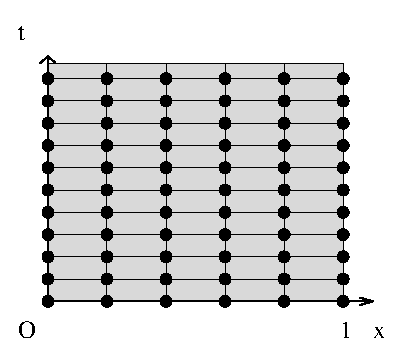
\includegraphics[height=5cm]{postscript/Figure1.ps}
  \end{center}
  \caption{閉領域 $[0,1]\times[0,\infty)$ を格子で分割する}
  \label{fig:grid}
\end{figure}

%  空間変数 $x$ の区間 $[0,1]$ を $N$ 等分して、等分点を $\{x_i; i=0,
%\cdots,N\}$ としよう。すなわち、\textbf{刻み幅} (stepsize) を $h=1/N$ 
%として、

  空間変数 $x$ の区間 $[0,1]$ を $N$ 等分して、等分点を $x_i$ ($i=0$,
$\cdots$, $N$) としよう。
すなわち、\textbf{刻み幅} (stepsize) を $h=1/N$ として、
%
\begin{equation}
  x_i = i h\quad\hbox{($i=0,1,\cdots,N$)}.
\end{equation}
%
とおく。
次に時間変数 $t$ に関する刻み幅 $\tau$ ($>0$) を$1$つ定めて、
%
\begin{equation}
  t_n=n\tau \quad\hbox{($n=0,1,2,\cdots$)}
\end{equation}
%
とおく。

% HANSEI
%  次の段落 (第10回、20分30秒〜23分0秒)
%  式 (16), (17) の最初の原稿が間違っていた。
%  このうち録音では (16) を読み上げてしまった。
%  訂正すべきかどうか。

  格子点 $(x_i,t_n)$ において、
$\dsp\frac{\rd u}{\rd t}$ を前進差分近似、
$\dsp\frac{\rd^2u}{\rd x^2}$ を $2$ 階中心差分近似すると、
%
\begin{align}
  &\frac{\rd u}{\rd t}(x_i,t_n)=\frac{u_{i}^{n+1}-u_i^n}{\tau}+O(\tau)
  \quad\mbox{($\tau\to +0$)},\\
  &\frac{\rd^2u}{\rd x^2}(x_i,t_n)
  =\frac{u_{i+1}^n-2u_{i}^n+u_{i-1}^{n}}{h^2}+O(h^2)\quad\mbox{($h\to +0$)}
\end{align}
%
となる。$u$ は熱伝導方程式 (\ref{eq:heat}) を満たすので、
$h$ と $\tau$ が十分小さいとき、
\begin{equation}
  \frac{u_{i}^{n+1}-u_{i}^{n}}{\tau}\kinji
  \frac{u_{i+1}^{n}-2u_{i}^{n}+u_{i-1}^{n}}{h^2}
\end{equation}
がなりたつ。

  そこで
%
\begin{equation}
    \frac{U_{i}^{n+1}-U_{i}^{n}}{\tau}
    = \frac{U_{i+1}^{n}-2U_{i}^{n}+U_{i-1}^{n}}{h^2}
    \label{eq:f-diff-eq0}
\end{equation}
%
という方程式を考え、
この方程式の解 $\{U_i^n\}$ を、
$\{u_i^n\}$ の近似値 (もとの熱方程式の初期値境界値問題の\textbf{近似解})
に採用することにする。

このような、未知数列に関する方程式で、
差分を含む方程式を\textbf{差分方程式}という\footnote{「差分」とは何?
という素朴な疑問に対して、きちんと回答するのは結構難しい。
広辞苑によると「変数のとる一連の数値に対応して関数のとる値の差」
とのことだが、
例えば $F_n=F_{n-1}+F_{n-2}$ のような Fibonacci 数列を定義する
「漸化式」も差分方程式と呼ばれる。}。
また差分方程式の解 $U_i^n$ を差分解という。

\begin{center}
  差分解 $=$ 差分方程式の解 $=$ $\{u_i^n\}$ の近似値 $=$ もとの方程式の近似解
\end{center}

%
ここで添字 $n$ は $0$ 以上の任意の整数に対して意味があるが、
$i$ については $U_{i-1}^{n}$, $U_{i+1}^{n}$ が現れるため、
$i=0,N$ に対して  (\ref{eq:f-diff-eq0}) を考えることはできず、
$1\leqq i\leqq N-1$ となることに注意しよう。
分母を払って $\lambda=\tau/h^2$ とおくと
%
\begin{equation}
    U_{i}^{n+1}-U_{i}^{n} = \lambda (U_{i+1}^{n}-2U_{i}^{n}+U_{i-1}^{n}).
\end{equation}

移項して
%
\iffalse
\begin{eqnarray}
  U_{i}^{n+1}&=&(1-2\lambda)U_i^n+\lambda\left(U_{i-1}^{n}+U_{i+1}^{n}\right)\\
&& \qquad\qquad\qquad\mbox{($1\leqq i\leqq N-1$; $n=0,1,\cdots$)}
\nonumber
\end{eqnarray}
\else
\begin{equation}
  U_{i}^{n+1}
  =(1-2\lambda)U_i^n+\lambda\left(U_{i-1}^{n}+U_{i+1}^{n}\right)
  \quad\text{($1\leqq i\leqq N-1$; $n=0,1,\cdots$)}
\end{equation}
\fi
%
となる。

  一方境界条件 (\ref{eq:D-bound}) に対応して
%
\begin{equation}
    U_{0}^{n}=U_{N}^{n}=0 \quad\text{($n=1,2,\cdots$)},
\end{equation}
%
初期条件 (\ref{eq:init}) に対応して
%
\begin{equation}
    U_{i}^{0}=f(x_i) \quad\text{($0\leqq i\leqq N$)}
\end{equation}
%
を考えるのは自然であろう。

  以上をまとめると、熱伝導方程式の初期値境界値問題 \DP に対応して、未
知数列 $\left\{U_i^n; 0\leqq i \leqq N, n\ge 0\right\}$ に関する方程式系
%
\begin{align}
  &U_{i}^{n+1}= (1-2\lambda)U_i^n+\lambda\left(U_{i-1}^{n}+U_{i+1}^{n}\right)
   \label{eq:f-diff-eq}
      \quad \text{($1\leqq i\leqq N-1; n=0,1,\cdots$)} \\
  &U_{0}^{n}=U_{N}^{n}=0 \qquad \text{($n=1,2,\cdots$)}
   \label{eq:BOUND} \\
  &U_{i}^{0}=f(x_i) \qquad \text{($0\leqq i\leqq N$)}
   \label{eq:INIT}
\end{align}
%
が得られる。

  この方程式の解 $\{U_i^n; 0\leqq i\leqq N, n\geqq 0\}$ は次のようにして
計算することができる。
%
\begin{enumerate}
\item
  右肩の添字 $n$ が $0$ の部分 $\{U_{i}^n; 0\leqq i\leqq N\}$ については、
(\ref{eq:INIT}) により値を求める。
%
\item
  $n=0,1,\cdots$ の順に次の手順で $\{U_{i}^{n+1}; 0\leqq i\leqq N\}$ を求める。
  \begin{enumerate}
    \item $1\leqq i\leqq N-1$ に
ついて $U_i^{n+1}$ を (\ref{eq:f-diff-eq}) で求める。
    \item $i=0,N$ については (\ref{eq:BOUND}) により $U_{0}^{n+1}
=U_{N}^{n+1}=0$.
  \end{enumerate}
\end{enumerate}

この方法は\textbf{前進 Euler 法}と呼ばれる。あるいは、差分方程式が 
$U_i^{n+1}$ について閉じた式 (それを求めるために方程式を解く必要がない) 
になっていることを前面に出して、\textbf{陽解法}または\textbf{陽的差分法}
と呼ぶことも多い。

%差分方程式の構成、
%一意可解性、プログラム(?)
%
\section{数値実験例}\label{sec:simulation}

  前節で導いた計算式に基づいて、
実際にコンピューターで計算してみた結果を紹介しよう。

\subsection*{(1) 解析解との比較}\label{subseq:comparison}
\addcontentsline{toc}{subsection}{(1) 解析解との比較}

  偏微分方程式の問題に対して、差分法で求めた近似解、すなわち差分方程式
の解のことを\textbf{差分解}とよび、それに対して元の偏微分方程式の解の
ことを\textbf{厳密解}とよぶ。厳密解は、それを解析的に
表示した (式で表した) 場合 
\textbf{解析解}ともよばれる。

  ここでは初期値境界値問題 \DirichletProblem の解析解 $u$ が簡単に求ま
る場合について、その解析解と差分解を比べてみよう。初期条件の関数 $f$ 
を $f(x)=f_0(x)\equiv\sin\pi x$ とすると、解 $u$ は
%
\begin{equation}
   u(x,t)=e^{-\pi^2 t}\sin\pi x
  \label{eq:exact}
\end{equation}
%
となる。このことは、第6章で扱った公式
%
\begin{equation}
    u(x,t)=
      \dsp\sum_{k=1}^\infty b_k e^{-k^2\pi^2 t}\sin k\pi x,
   \quad
   b_k=2\dsp\int_0^1 f(x)\sin k\pi x\;\Dx \quad\text{($k=1,2,\cdots$)}
  \label{eq:sol}
\end{equation}
%
中の係数 $b_k$ を計算して $b_1=1$, $b_k=0$ ($k=2,3,\cdots$) となること
を示してもよいし、 (\ref{eq:exact}) で定義される $u$ が \DP を満足する
ことを直接代入して確かめてもよい。
表 \ref{tbl:test1} は $(x,t)=(1/2,0.1)$ にお
ける値 $u(1/2,0.1)=\exp(-0.1\pi^2)\sin(\pi/2)=0.372707838\cdots$ に対する
近似値を並べてみたものである。これを見ると、誤差が $N$ の増加とともに
減少して行っているのがよくわかる。図 \ref{fig:error} は
その様子を両側対数グラフに表したものである (対数グラフの読み方については、
補足の (2) にまとめておいた)。グラフの横軸が $N$ で、縦軸が相対誤差を表す。
このグラフから、誤差は $N^{-2}$ に比例していると推察できる。
\par
%
% TABLE 2
\iffalse
\begin{table}
  %\begin{minipage}[t]{.47\textwidth}
    \centering
    \begin{tabular}{|c|c|c|}\hline
      $N$ & $u(1/2,0.1)$ の近似値 & 相対誤差(\%) \\ \hline
        10& 0.366544& 1.653709 \\
        20& 0.371188& 0.407728 \\
        30& 0.372034& 0.180753 \\
        40& 0.372329& 0.101583 \\
        50& 0.372466& 0.064987 \\
        60& 0.372540& 0.045120 \\
        70& 0.372584& 0.033145 \\
        80& 0.372613& 0.025374 \\
        90& 0.372633& 0.020048 \\
       100& 0.372647& 0.016238 \\ \hline
    \end{tabular}
    \caption{$(x,t)=(1/2,0.1)$ で値の変化}\label{tbl:test1}
  %\end{minipage}
\end{table}
\else
\begin{table}
  %\begin{minipage}[t]{.47\textwidth}
    \centering
    \begin{tabular}{|c|c|c|}\hline
      $N$ & $u(1/2,0.1)$ の近似値 & 相対誤差(\%) \\ \hline
  10 &0.36654433 &1.653709\\
  20 &0.37118820 &0.407728\\
  40 &0.37232923 &0.101583\\
  80 &0.37261327 &0.025374\\
 160 &0.37268420 &0.006342\\
 320 &0.37270193 &0.001585\\
 640 &0.37270636 &0.000396\\
\hline
    \end{tabular}
    \caption{$(x,t)=(1/2,0.1)$ で値の変化 ($\lambda=1/2$).}\label{tbl:test1}
  %\end{minipage}
\end{table}
\fi
% FIGURE 2
\begin{figure}
  %\begin{minipage}[t]{.47\textwidth}
  \centering
%  \begin{center}
%    最初 test1.ps は ``%'' のままでやっていたのだが、対数グラフを描くのに
%    ``%'' も変な感じがする、というので、単に比をそのままプロットした
%    のが new-test1.ps
%    \epsfile{file=postscript/test1.ps,width=7cm}
    %\epsfile{file=postscript/new-test1.ps,width=7cm}
    %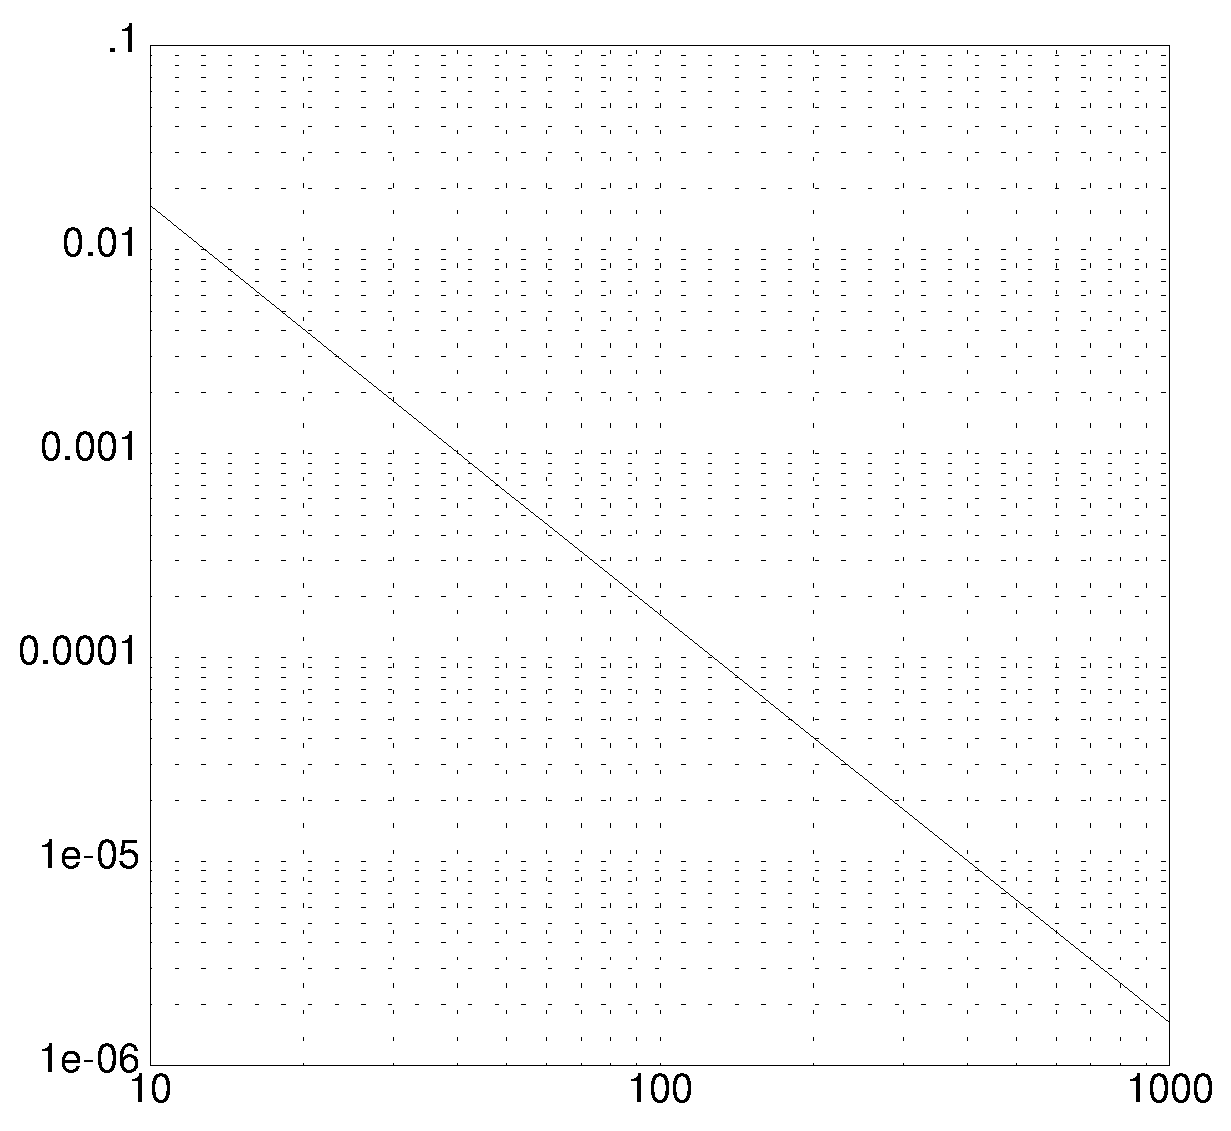
\includegraphics[width=7cm]{postscript/new-test1.ps}
    %\includegraphics[width=7cm]{eps/figure2.eps}
   \includegraphics[width=7cm]{eps/test1.eps}
%  \end{center}
  \caption{$(x,t)=(1/2,0.1)$ での相対誤差の変化 ($\lambda=1/2$).}
  \label{fig:error}
  %\end{minipage}
\end{figure}

\subsection*{(2) 解の漸近挙動}
\addcontentsline{toc}{subsection}{(2) 解の漸近挙動}

  時刻 $t$ を $t\to+\infty$ とした場合の $u(\cdot,t)$ の振る舞いのことを、
解の\textbf{漸近挙動}とよぶ。

\subsubsection*{<ディリクレ (Dirichlet) 境界条件の場合>}

% 実は、録音で、「(28)の右辺の」というべきところを、「(29)の右辺の」
% と言い間違えた。

  初期値境界値問題 \DirichletProblem の解の公式
% (28)
\begin{equation}
    u(x,t)=
	\sum_{k=1}^\infty b_k e^{-k^2\pi^2 t}\sin k\pi x, \quad
    b_k=2\dsp\int_0^1 f(x)\sin k\pi x\;\Dx \quad\text{($k=1,2,\cdots$)}
\end{equation}
%
から、$t\to\infty$ とすると、$u$ は定数関数 $0$ に収束することがわかる:
% (29)
\begin{equation}\label{eq:uは0に収束する}
  \lim_{t\to\infty} u(x,t)=0 \quad\text{($0\leqq x \leqq 1$)}.
\end{equation}
(式 (\ref{eq:uは0に収束する}) の厳密な証明は、補足 (3) にまとめておいた。)

  このことを、初期条件の関数 $f$ が
% (30)
\begin{equation}
f_1(x)=\left\{
  \begin{array}{cl}
    x & \left(0\leqq x\leqq \dsp\half\right) \\
   \noalign{\vspace{1ex}}
   1-x & \left(\dsp\half\leqq x\leqq 1\right)
  \end{array}
  \right.
\end{equation}
%
である場合 (グラフは図 \ref{fig:func1}) に、差分法で 
\DirichletProblem を解いて、確かめてみよう。$N=50$, $\lambda = 1/2$ と
して解いた結果を描いたのが図 \ref{fig:test2a} 〜 
\ref{fig:test2d} である。それぞれの図は、
一つの固定された $n$ の値に対する $\{U_{i}^{n};
0\leqq i\leqq N\}$ の値をもとにして描かれている。
すなわち、$t=n\tau= 0.01$, $0.02$, $0.03$,
$0.04$ としたときの $x$ の関数 $u(x,t)$ のグラフに対応するものである。
グラフの横軸が位置、縦軸が温度を表していることを考えると、
時間が経つにつれて、
温度の高いところから低いところへ熱が流れていく様子がわかる。
図 \ref{fig:test2} は $t=0$ から $t=0.3$ まで $0.01$ 刻みの時刻におけるグラフをまとめて描
いてみたものである。時間が経つにつれて、
温度が $0$ に近付いていくのがわかる。
%
\begin{figure}
  \centering
  \begin{minipage}[t]{0.3\textwidth}
    %\epsfile{file=postscript/func1.ps,width=5cm}
    %\includegraphics[width=5cm]{postscript/func1.ps}
     \includegraphics[width=5cm]{eps/figure3.eps}
    \caption{初期条件 $f=f_1$}\label{fig:func1}
  \end{minipage}
  \hfill
  \begin{minipage}[t]{0.3\textwidth}
    %\epsfile{file=postscript/test2a.ps,width=5cm}
    %\includegraphics[width=5cm]{postscript/test2a.ps}
     \includegraphics[width=5cm]{eps/figure4.eps}
    \caption{$t=0.01$}\label{fig:test2a}
  \end{minipage}
  \hfill
  \begin{minipage}[t]{0.3\textwidth}
    %\epsfile{file=postscript/test2b.ps,width=5cm}
    %\includegraphics[width=5cm]{postscript/test2b.ps}
     \includegraphics[width=5cm]{eps/figure5.eps}
    \caption{$t=0.02$}\label{fig:test2b}
  \end{minipage}
\end{figure}
%
\begin{figure}
  \begin{minipage}[t]{0.3\textwidth}
    %\epsfile{file=postscript/test2c.ps,width=5cm}
    %\includegraphics[width=5cm]{postscript/test2c.ps}
     \includegraphics[width=5cm]{eps/figure6.eps}

    \caption{$t=0.03$}\label{fig:test2c}
  \end{minipage}
  \hfill
  \begin{minipage}[t]{0.3\textwidth}
    %\epsfile{file=postscript/test2d.ps,width=5cm}
    %\includegraphics[width=5cm]{postscript/test2d.ps}
     \includegraphics[width=5cm]{eps/figure7.eps}
    \caption{$t=0.04$}\label{fig:test2d}
  \end{minipage}
  \hfill
  \begin{minipage}[t]{0.3\textwidth}
   %\epsfile{file=postscript/test2.ps,width=5cm}
   %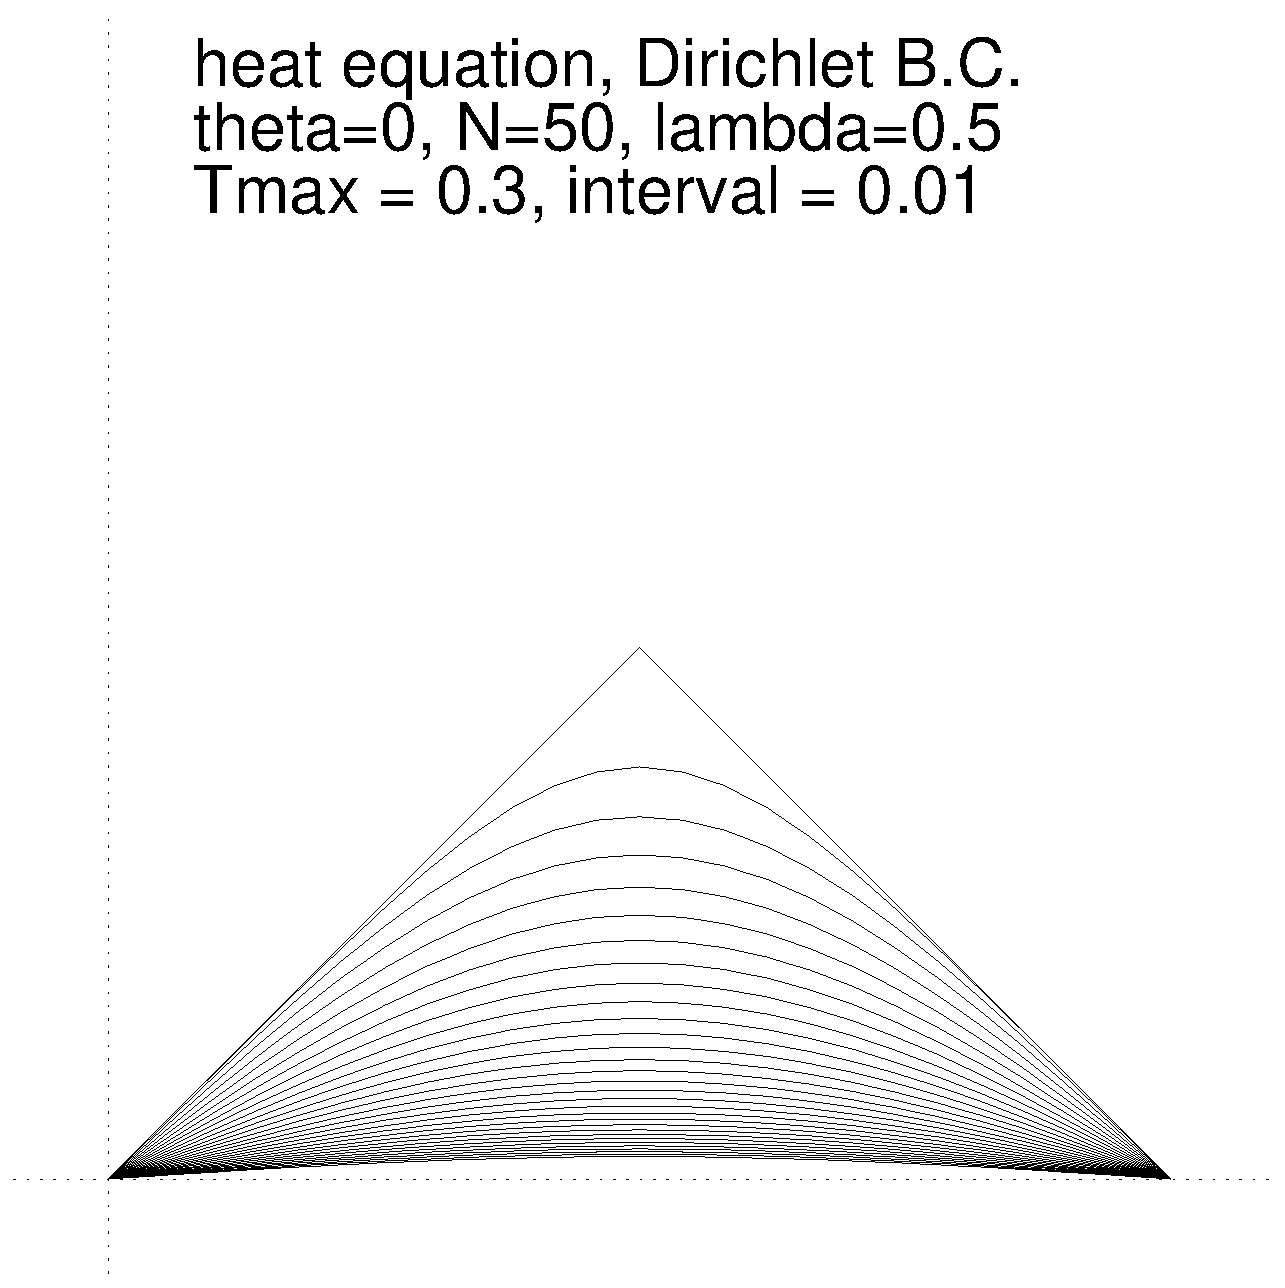
\includegraphics[width=5cm]{postscript/test2.ps}
     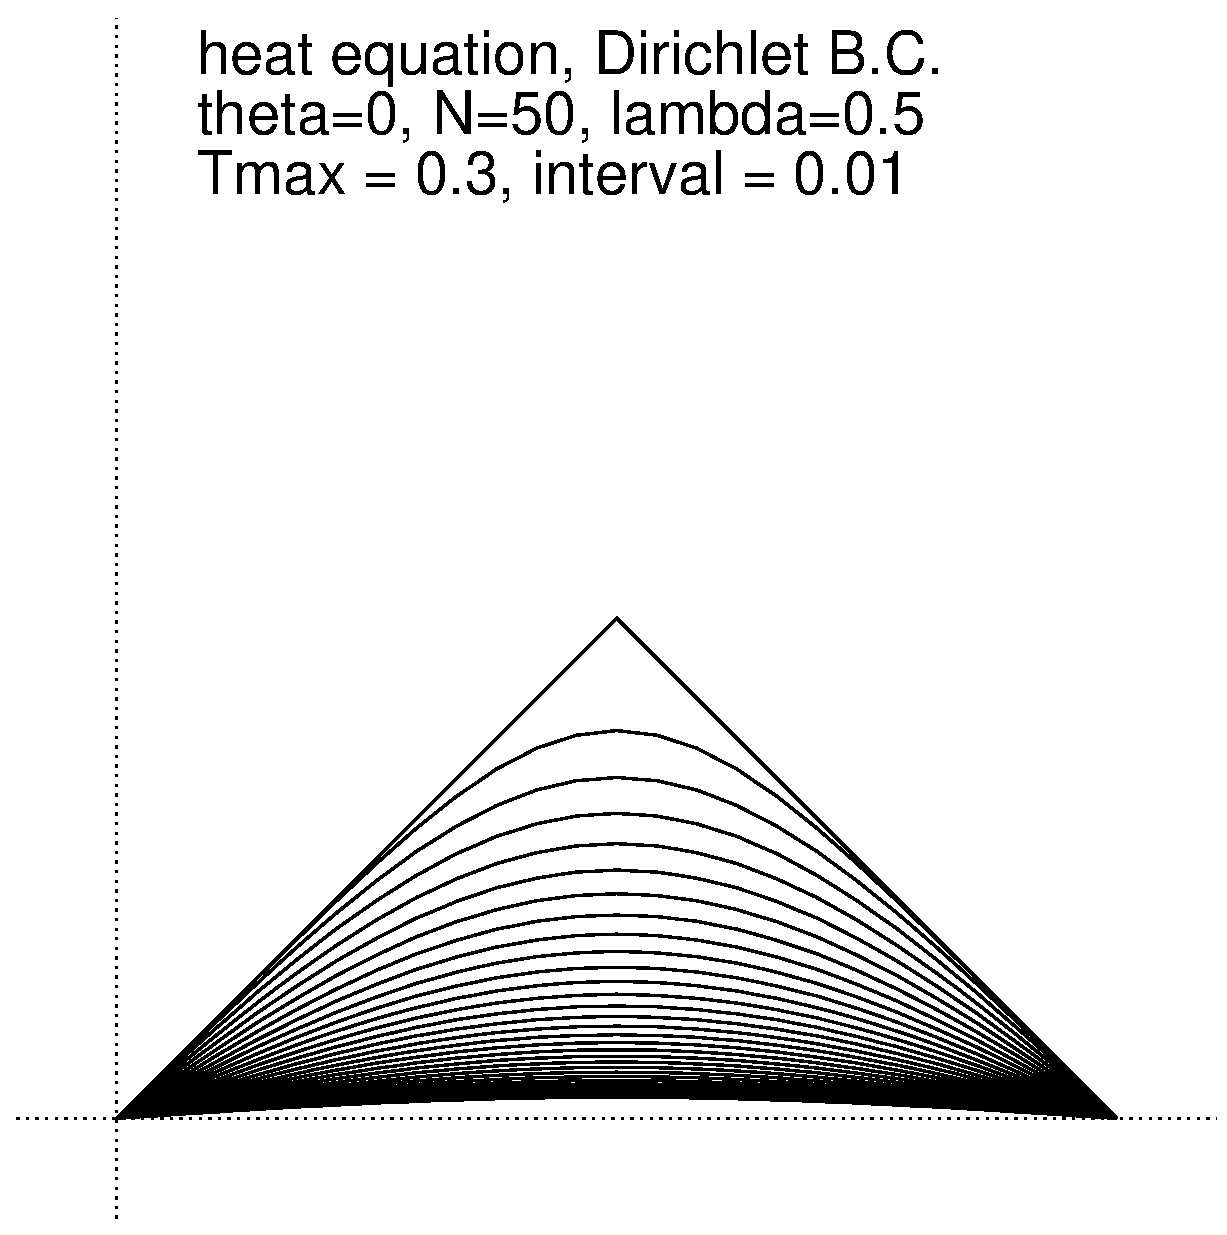
\includegraphics[width=5cm]{eps/figure8.eps}
   %\caption{Dirichlet 条件の場合の漸近挙動}\label{fig:test2}
    \caption{ディリクレ条件, $t=0\sim 0.3$, $\Delta t=0.01$}\label{fig:test2}
  \end{minipage}
\end{figure}

\subsubsection*{<ノイマン (Neumann) 境界条件の場合>}

  ここでは境界条件を同次ディリクレ境界条件 (\ref{eq:D-bound}) から、
同次ノイマン境界条件
%
\begin{equation}
  u_x(0,t)=u_x(1,t)=0 \quad\hbox{($t>0$)}
  \label{eq:N-bound}
\end{equation}
%
に変えた問題を考えよう。第 6 章と同様の計算により、
%
\begin{equation}
    u(x,t)=
      \half a_0+
      \sum_{k=1}^\infty a_k e^{-k^2\pi^2 t}\cos k\pi x, \quad
    a_k=2\dsp\int_0^1 f(x)\cos k\pi x\;\Dx \quad\hbox{($k=0,1,\cdots$)}
\end{equation}
%
を導くことができる。この公式から、$t\to\infty$ とすると、
$u$ はある定数関数に収束することがわかる:
%
\begin{equation}
  \lim_{t\to\infty} u(x,t) = 
    \dfrac{a_0}{2} \quad\hbox{($0\leqq x\leqq 1$)}.
\end{equation}
%
\begin{figure}
\centering
\begin{minipage}[t]{0.30\textwidth}
  %\epsfile{file=postscript/test3a.ps,width=5cm}
  %\includegraphics[width=5cm]{postscript/test3a.ps}
   \includegraphics[width=5cm]{eps/figure9.eps}
  \caption{$t=0$}\label{fig:test3a}
\end{minipage}
\hfill
\begin{minipage}[t]{0.30\textwidth}
  %\epsfile{file=postscript/test3b.ps,width=5cm}
  %\includegraphics[width=5cm]{postscript/test3b.ps}
   \includegraphics[width=5cm]{eps/figure10.eps}
  \caption{$t=0.01$}\label{fig:test3b}
\end{minipage}
\hfill
\begin{minipage}[t]{0.30\textwidth}
  %\epsfile{file=postscript/test3c.ps,width=5cm}
  %\includegraphics[width=5cm]{postscript/test3c.ps}
   \includegraphics[width=5cm]{eps/figure11.eps}
  \caption{$t=0.02$}\label{fig:test3c}
\end{minipage}
\end{figure}
%
\begin{figure}
\centering
\begin{minipage}[t]{0.30\textwidth}
  %\epsfile{file=postscript/test3d.ps,width=5cm}
  %\includegraphics[width=5cm]{postscript/test3d.ps}
   \includegraphics[width=5cm]{eps/figure12.eps}
  \caption{$t=0.04$}\label{fig:test3d}
\end{minipage}
\hfill
\begin{minipage}[t]{0.30\textwidth}
  %\epsfile{file=postscript/test3e.ps,width=5cm}
  %\includegraphics[width=5cm]{postscript/test3e.ps}
   \includegraphics[width=5cm]{eps/figure13.eps}
  \caption{$t=0.05$}\label{fig:test3e}
\end{minipage}
\hfill
\begin{minipage}[t]{0.30\textwidth}
  %\epsfile{file=postscript/test3.ps,width=5cm}
  %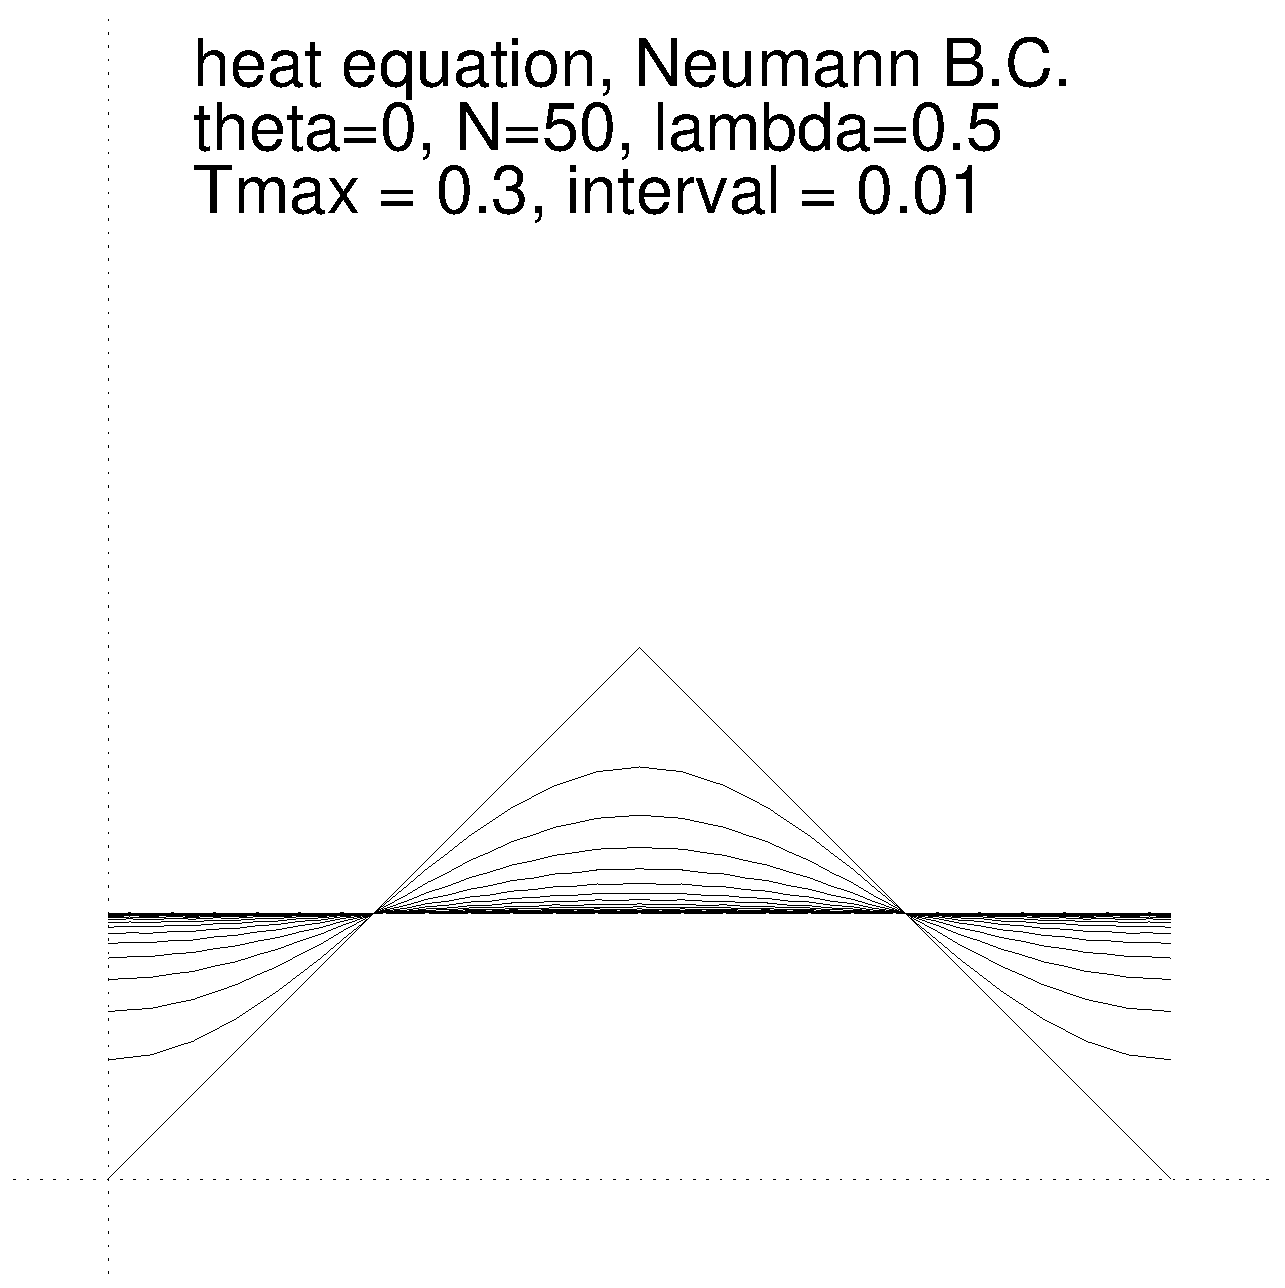
\includegraphics[width=5cm]{postscript/test3.ps}
   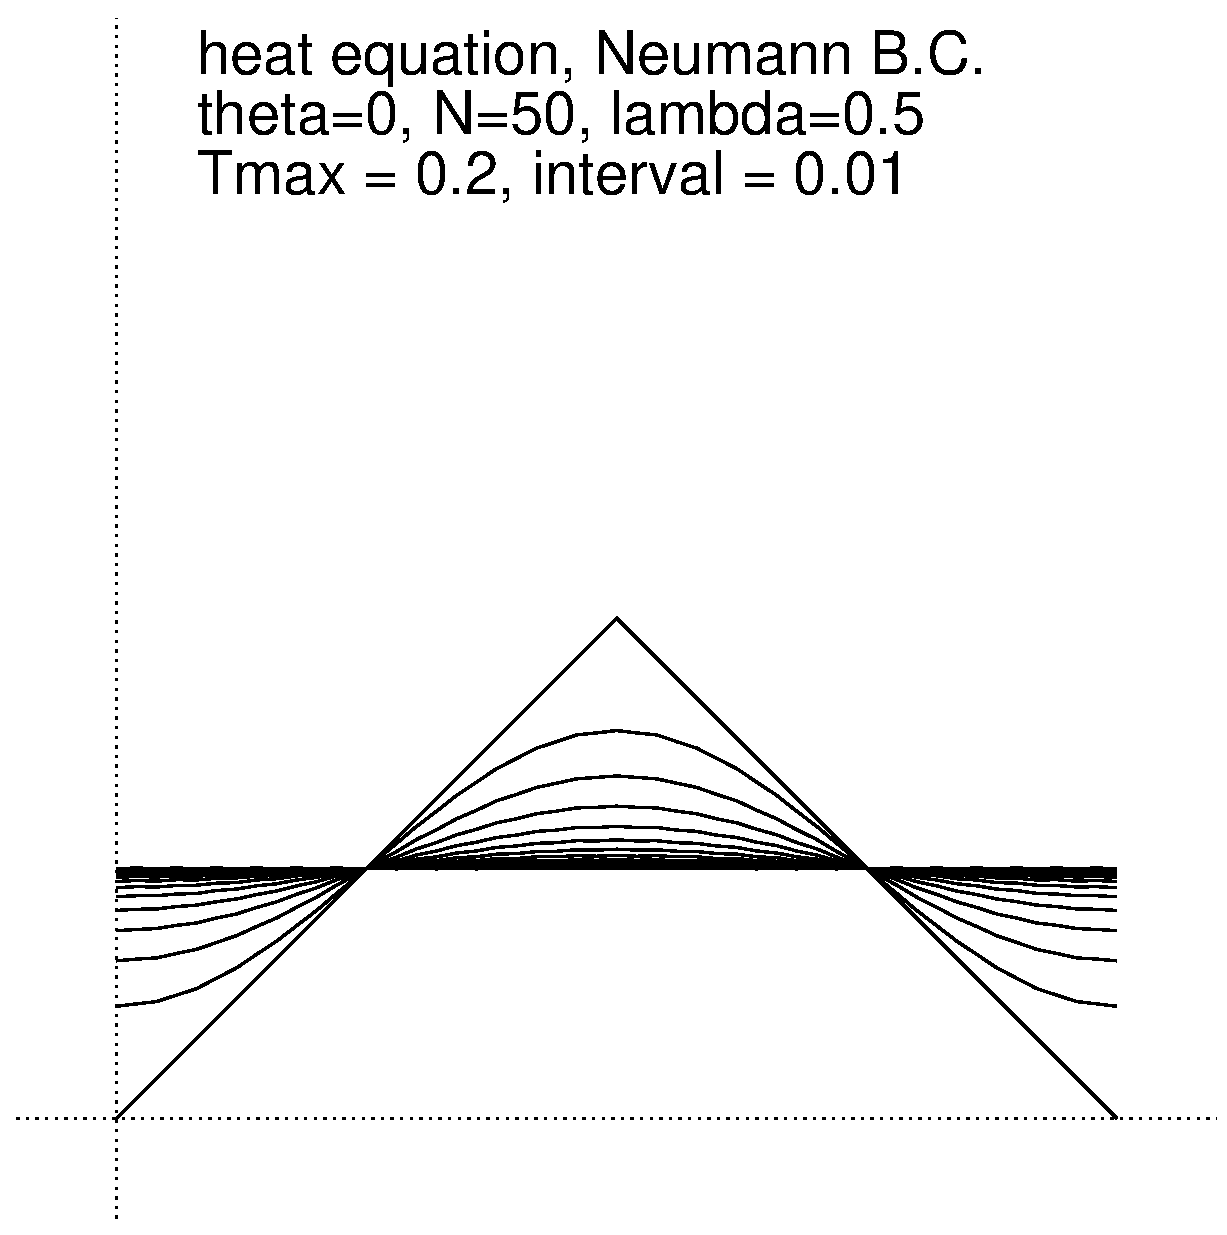
\includegraphics[width=5cm]{eps/figure14.eps}
  \caption{$t=0\sim 0.2$}\label{fig:test3}
\end{minipage}
\end{figure}
%

  図 \ref{fig:test3a}〜\ref{fig:test3e} では、
初期条件は $f_1$ のままで、
境界条件を同次ノイマン境界条件にした問題を、
$N=50$, $\lambda=1/2$ の差分法で解いた場合の計算結果を示したものである。
確かに時間が経つにつれて $u(\cdot,t)$ は定数関数に収束して行く様子がわかる。
さらにその値についても調べてみよう。 $f=f_1$ に対して、
%
% HANSEI
%   次の式で、「図 \ref{fig:func1}のグラフ」すなわち
%  「図7-3のグラフ」としたが、「図7-9のグラフ」とした方が良かった。
%  まあ、間違いではない。
\begin{equation}
  \quad\dfrac{a_0}{2}=\int_0^1f_1(x)\;\Dx=
  %\hbox{図 \ref{fig:func1}のグラフと $x$ 軸の囲む三角形領域の面積}=\frac{1}{4}
  \hbox{図 \ref{fig:func1}のグラフと $x$ 軸の囲む三角形の面積}=\frac{1}{4}
\end{equation}
%
であるが、数値解の値は表 \ref{tbl:test3} のようになっていて、
解析解と同様に $1/4=0.25$ へ収束して行く様に見える。
(問題が対称なので、区間の左半分の値のみを示してある。)

\begin{table}
  %\begin{minipage}[t]{.47\textwidth}
    \centering
    \begin{tabular}{|c|c|c|c|c|c|c|}\hline
\diagbox{$t$}{$x$} & $0$& $0.1$& $0.2$& $0.3$& $0.4$& $0.5$ \\ \hline
0.00&0.000000&0.100000&0.200000&0.300000&0.400000&0.500000\\
0.05&0.221849&0.227225&0.241301&0.258699&0.272775&0.278151\\
0.10&0.246121&0.246862&0.248801&0.251199&0.253138&0.253879\\
0.15&0.249466&0.249568&0.249835&0.250165&0.250432&0.250534\\
0.20&0.249926&0.249940&0.249977&0.250023&0.250060&0.250074\\
0.25&0.249990&0.249992&0.249997&0.250003&0.250008&0.250010\\
0.30&0.249999&0.249999&0.250000&0.250000&0.250001&0.250001\\
0.35&0.250000&0.250000&0.250000&0.250000&0.250000&0.250000\\
0.40&0.250000&0.250000&0.250000&0.250000&0.250000&0.250000\\\hline
    \end{tabular}
    \caption{定数定常解への収束 (ノイマン境界条件, $\theta=0$,
  $N=40$, $\lambda=0.5$)}\label{tbl:test3}
  %\end{minipage}
\end{table}

\subsection*{(3) 熱伝導方程式の平滑化作用、$t\to\infty$ の際の漸近形}
\addcontentsline{toc}{subsection}
{\texorpdfstring{(3) 熱伝導方程式の平滑化作用、$t\to\infty$ の際の漸近形}
                {(3) 熱伝導方程式の平滑化作用、t→∞ の際の漸近形}}

  既に何回か、「熱は温度の高いところから低いところへ流れる」ので、
温度の高いところは低くなり、温度の低いところは高くなる、
ことを見て来ているが、より詳しく分析することにしよう。
%

\medskip
\noindent\textbf{微分可能性とフーリエ係数の減衰}

  第 6 章で関数 $f$ のフーリエ級数
%
\[
  \frac{a_0}{2}+\sum_{k=1}^\infty
  (a_k \cos k\pi x+ b_k \sin k\pi x),
\]
%
の収束には、$f$ の滑らかさ (微分可能性) が関係することに言及した。
実は関数 $f$ が滑らかなほど、フーリエ係数 $a_k$, $b_k$ の絶対値 $|a_k|$,
$|b_k|$ は $k$ が増加するにつれてより速く減衰することがわかっている。
たとえば、具体的には次のような事実がある:
%
\begin{equation}
  \text{$f$ が $C^\ell$ 級 ($\ell$ 回連続的微分可能)}
  \quad\Longrightarrow\quad
  \text{$a_k,b_k=o(k^{-\ell})$ \quad ($k\to+\infty$)}.
  \label{eq:fのフーリエ係数の減衰}
\end{equation}

  また、これとは逆に、$f$ のフーリエ係数がより速く減衰するならば、
$f$ はより高い微分可能性をもつ (=より多い回数微分できる) こともわかっている。
実際
%
\begin{equation}
  \dsp\sum_{k=1}^\infty k^\ell(|a_k|+|b_k|)<\infty\quad 
  \Longrightarrow\quad \text{$f$ は $C^\ell$ 級}.
\end{equation}

  それでは、
$f$ が図 \ref{fig:test4a} のような、
たくさんの\Ruby{かど}{角}のあるグラフを持つ関数 $f_2$ の場合にはどうなるであろうか?
この場合は、角となっている点で $f$ は微分できないので、
$k\to+\infty$ のときの $|a_k|$, $|b_k|$ の減衰はゆっくりである\footnote
{具体的には、$a_k,b_k=o(1)$ ($k\to\infty$) であるが、
$\dsp\sum_{k=1}^\infty k\left(\left|a_k\right|+\left|b_k\right|\right)
=\infty$ である。}。
この $f=f_2$ を初期値としたときの \DirichletProblem の解を考えよう。
解の公式 (\ref{eq:sol}) を見ると、第 $k$ 項には、
時間に関係する因子 $\exp\left(-k^2\pi^2t\right)$ がかかっていて、
これは $t>0$ のとき、$k$ の増加につれ急激に小さくなる。
従って、初期条件 $f=f_2$ が低い微分可能性しか持っていなくても、
少しでも時間が経過すると、
$u$ は高い微分可能性をもつ (実は無限回微分可能になる) ことが導かれる。

  実際に $f=f_2$ を初期データとした問題を差分法で解いた結果が
図 \ref{fig:test4a} 〜 \ref{fig:test4} である。
これによると、すでに $t=0.001$ という早い段階で角が消滅している
ことがわかる。

\medskip
\noindent\textbf{凹凸の消滅}

  さらに時間が経過するにつれ、
凹凸の激しいところほど急速に変形して消滅し、
グラフが平滑な形に近づくことが見てとれる。
凹凸が激しい (変化が急) なところがあるのは、
大きな番号 $k$ に対する $\sin k\pi x$ の項が大きな割合を
占めているからであると推測できる。
しかし $k$ が大きいほど、
時間に関係する因子 $\exp \left(-k^2\pi^2t \right)$ は、
$t$ の増加につれて速く小さくなる。
そのため、凹凸の変化が激しいところほど早く消滅する、
と考えられる。

\medskip
\noindent\textbf{漸近形}

  公式 (\ref{eq:sol}) において、$t$ が非常に大きくなると、 $k=2$, $3$,
$\cdots$ の項は、
$k=1$ に対応する項 $b_1\exp(-\pi^2 t)\sin \pi x$ に比べて
無視できるほど小さくなることがわかる。すなわち $t$ が大きいところでは、
%
\begin{equation}
   u(x,t)\kinji b_1 e^{-\pi^2t}\sin \pi x.
\end{equation}
%
これはグラフでいうと、形がサイン・カーブの半周期分に近づくこと
を意味する。実際、図 \ref{fig:test4} ではそうなっている。

%
\begin{figure}[hbtp]
\centering
\begin{minipage}[t]{0.30\textwidth}
  %\epsfile{file=postscript/test4a.ps,width=5cm}
  %\includegraphics[width=5cm]{postscript/test4a.ps}
  \includegraphics[width=5cm]{eps/figure15.eps}
  \caption{$t=0$}\label{fig:test4a}
\end{minipage}
\hfill
\begin{minipage}[t]{0.30\textwidth}
  %\epsfile{file=postscript/test4b.ps,width=5cm}
  %\includegraphics[width=5cm]{postscript/test4b.ps}
  \includegraphics[width=5cm]{eps/figure16.eps}
  \caption{$t=0.001$}\label{fig:test4b}
\end{minipage}
\hfill
\begin{minipage}[t]{0.30\textwidth}
  %\epsfile{file=postscript/test4c.ps,width=5cm}
  %\includegraphics[width=5cm]{postscript/test4c.ps}
  \includegraphics[width=5cm]{eps/figure17.eps}
  \caption{$t=0.002$}\label{fig:test4c}
\end{minipage}
%\end{figure}
%%
%\begin{figure}
%\centering
%\hfill
\begin{minipage}[t]{0.30\textwidth}
  %\epsfile{file=postscript/test4d.ps,width=5cm}
  %\includegraphics[width=5cm]{postscript/test4d.ps}
  \includegraphics[width=5cm]{eps/figure18.eps}
  \caption{$t=0.003$}\label{fig:test4d}
\end{minipage}
\hfill
\begin{minipage}[t]{0.30\textwidth}
  %\epsfile{file=postscript/test4e.ps,width=5cm}
  %\includegraphics[width=5cm]{postscript/test4e.ps}
  \includegraphics[width=5cm]{eps/figure19.eps}
  \caption{$t=0.004$}\label{fig:test4e}
\end{minipage}
\hfill
\begin{minipage}[t]{0.30\textwidth}
  %\epsfile{file=postscript/test4.ps,width=5cm}
  %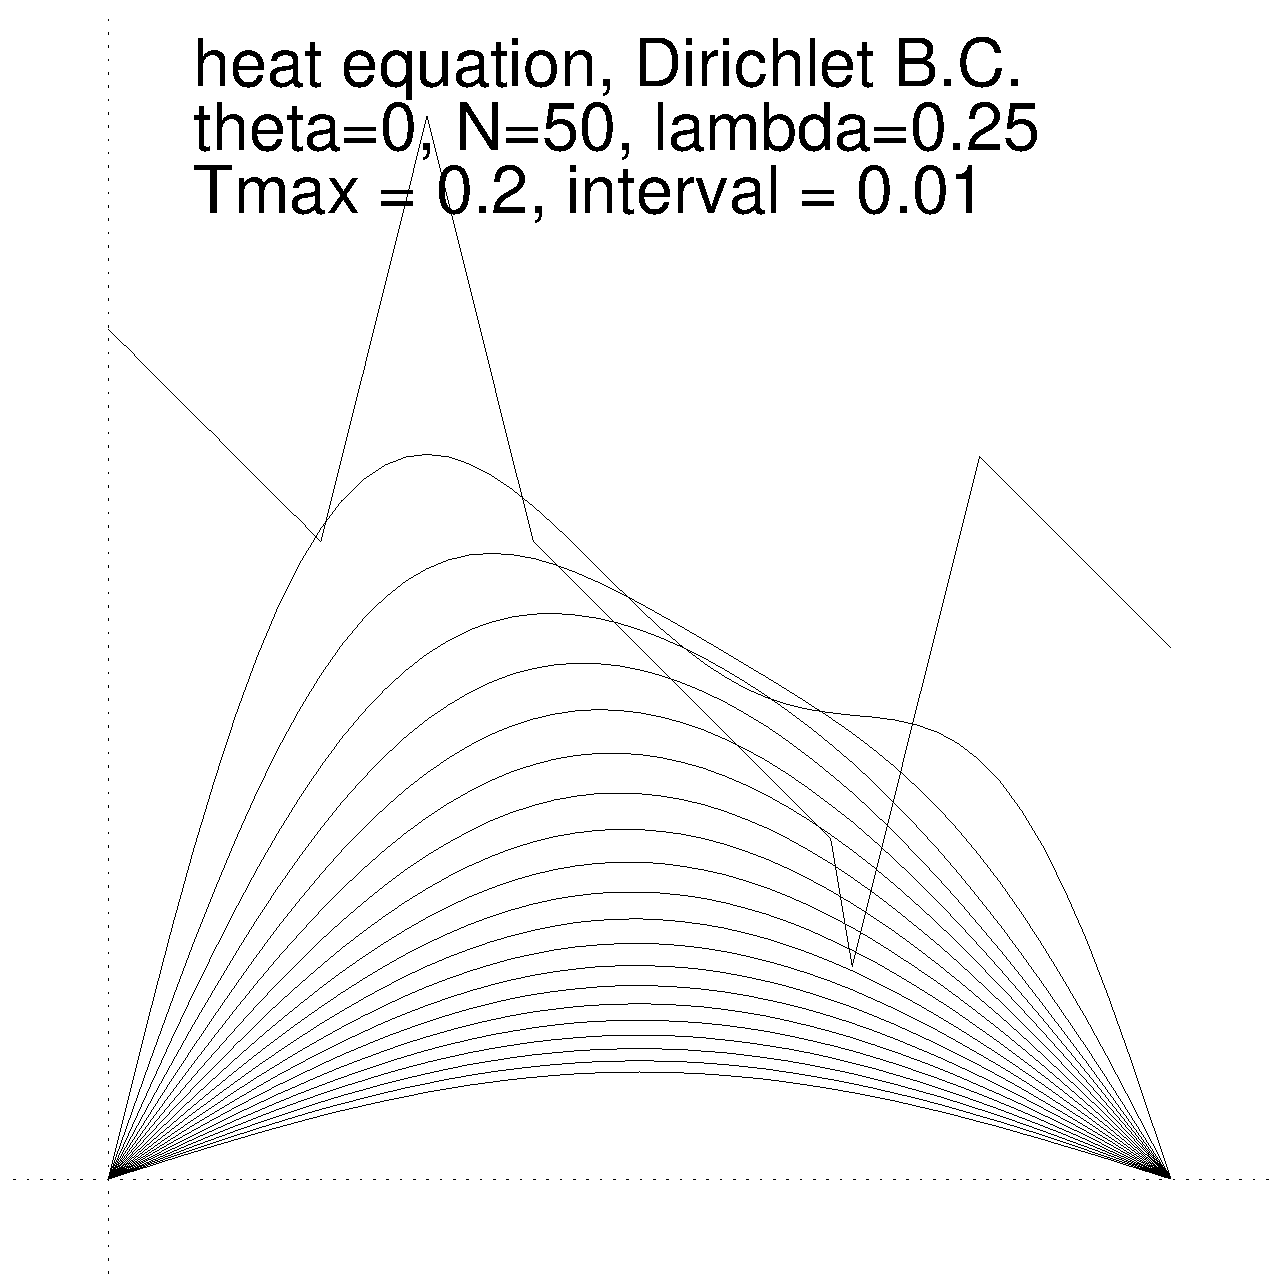
\includegraphics[width=5cm]{postscript/test4.ps}
  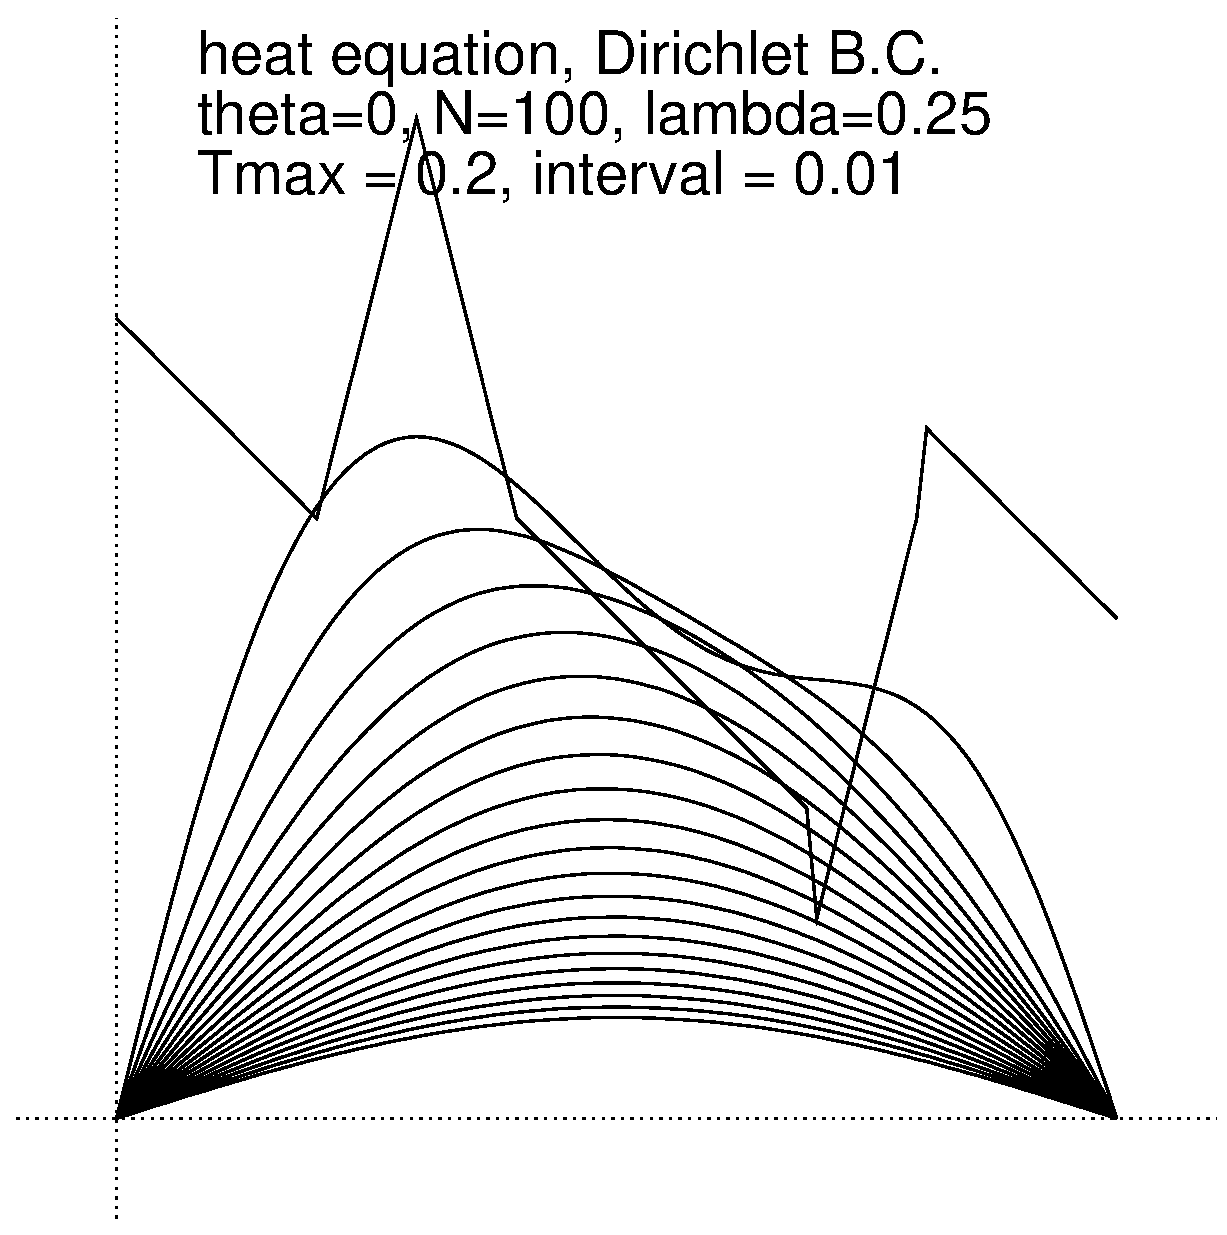
\includegraphics[width=5cm]{eps/figure20.eps}
  \caption{$t=0\sim 0.2, \Delta t=0.01$}\label{fig:test4}
\end{minipage}
\end{figure}

%
\section{陰解法}\label{sec:implicitscheme}

\subsection*{(1) 安定性}
\addcontentsline{toc}{subsection}{(1) 安定性}

  前節で示した計算結果は、素朴に検討したに過ぎないが、なかなか満足の出
来るものであった。ところが、うまく行かない場合もあることを見てみよう。

  前節では、いずれの計算例も $\lambda=\tau/h^2$ を $1/2$ あるいは 
$\lambda=1/4$ として計算したのであるが、 $\lambda=0.51$ として、 
$f=f_1$ の場合の初期値境界値問題 \DirichletProblem を解いたのが図 
\ref{fig:unst-a}〜\ref{fig:unst-d} である。解こうとしてい
る熱伝導方程式の初期値境界値問題自体は図 \ref{fig:test2a}〜
\ref{fig:test2d} と同じものなのだが、計算結果は似ても似つかない悲惨な
ものになっている。このような現象を\textbf{不安定現象}とよぶ。これに対
して、差分解の大きさが初期値、境界値で定まる定数 ($N$ にも依存しない) 
で押えられるとき、差分スキームは\textbf{安定}である、という。

  実は第 \ref{sec:f-diff-eq} 節で導いた差分方程式の解が、
安定に計算できるための必要十分条件は、
$\lambda$ が $0<\lambda\leqq 1/2$ を満たすことである、
ということがわかっている。実際、$0<\lambda\leqq 1/2$ のとき
\begin{equation}
  |U_{i}^{n}|\leqq \max_{x\in[0,1]}|f(x)|
  \quad\mbox{($0\leqq i\leqq N$; $n=0,1,\cdots$)}
\end{equation}
が成り立つ (補足 (5) 定理 \ref{th:maximum} 参照)。

  さらに、この条件 $0<\lambda\leqq 1/2$ が満たされる場合は、
任意に固定した正数 $T$ に対して
%
\begin{equation}
  \lim_{N\to\infty}\max_{\genfrac{}{}{0pt}{}{0\leqq i\leqq N}{0\leqq n\leqq T/\tau}}
    \left|u(x_i,t_n)-U_i^n\right|=0
\end{equation}
が成り立つこと、すなわち\textbf{差分解の厳密解への収束}も証明
できる (これについても、補足 (5) 定理 \ref{th:convergence} を参照)。
条件 $0\le i\le N$, $0\le n\le T/\tau$ は、
$(x_i,t_n)$ が $[0,1]\times[0,T]$ に含まれることを意味する。

\begin{figure}[hbtp]
\centering
\begin{minipage}[t]{0.30\textwidth}
  %\epsfile{file=postscript/unst-a.ps,width=5cm}
  %\includegraphics[width=5cm]{postscript/unst-a.ps}
  \includegraphics[width=5cm]{eps/figure21.eps}
  \caption{$t=0.009996$}\label{fig:unst-a}
\end{minipage}
\hfill
\begin{minipage}[t]{0.30\textwidth}
  %\epsfile{file=postscript/unst-b.ps,width=5cm}
  %\includegraphics[width=5cm]{postscript/unst-b.ps}
  \includegraphics[width=5cm]{eps/figure22.eps}
  \caption{$t=0.019992$}\label{fig:unst-b}
\end{minipage}
\hfill
\begin{minipage}[t]{0.30\textwidth}
  %\epsfile{file=postscript/unst-c.ps,width=5cm}
  %\includegraphics[width=5cm]{postscript/unst-c.ps}
  \includegraphics[width=5cm]{eps/figure23.eps}
  \caption{$t=0.029988$}\label{fig:unst-c}
\end{minipage}
\hfill
\begin{minipage}[t]{0.30\textwidth}
  %\epsfile{file=postscript/unst-d.ps,width=5cm}
  %\includegraphics[width=5cm]{postscript/unst-d.ps}
  \includegraphics[width=5cm]{eps/figure24.eps}
  \caption{$t=0.039984$}\label{fig:unst-d}
\end{minipage}
\end{figure}
%

\subsection*{(2) 後退 Euler 法}\label{sec:b-diff-eq}
\addcontentsline{toc}{subsection}{(2) 後退 Euler 法}

  前項では、第 \ref{sec:f-diff-eq} 節で導いた差分方程式の安定な計算
のためには $0<\lambda\leqq 1/2$ があれば十分であると述べたが、この条件
を保証しようとすると、計算量が大きく (=計算に要する時間が長く) なりが
ちである。これを緩和するための、重要な手法を紹介しておこう。

  第 \ref{sec:f-diff-eq} 節では、時間に関する偏導関数 $\dsp\frac{\rd u}{\rd t}$ を前進
差分近似したが、これを後退差分近似に置き換えて得られる
% (38)
\begin{equation}
    \frac{U_{i}^{n}-U_{i}^{n-1}}{\tau}
    = \frac{U_{i+1}^{n}-2U_{i}^{n}+U_{i-1}^{n}}{h^2}
   \quad\mbox{($1\le i\le N-1$, $n\ge 1$)}
\end{equation}
%
を考えよう。番号 $n$ を一つずらすと  ($n-1$ を $n$ と書き直すと)、これは
% (39)
\begin{equation}
    \frac{U_{i}^{n+1}-U_{i}^{n}}{\tau}
    = \frac{U_{i+1}^{n+1}-2U_{i}^{n+1}+U_{i-1}^{n+1}}{h^2}
   \quad\mbox{($1\le i\le N-1$, $n\ge 0$)}
    \label{eq:b-diff-eq0}
\end{equation}
%
となる。移項して、二番目の添字が $n$ であるものと、$n+1$ であるものと
を分離すると
%
\begin{equation}
  \label{eq:b-diff-eq}
  (1+2\lambda)U_{i}^{n+1}-\lambda\left(U_{i-1}^{n+1}+U_{i+1}^{n+1}\right)
  =U_{i}^{n}\quad
 \mbox{($1\leqq i\leqq N-1$, $n\ge 0$)}
\end{equation}
%
のような差分方程式が得られる。
この差分方程式にもとづいて差分解を定める方法を\textbf{後退 Euler 法}とよぶ。

(\ref{eq:b-diff-eq}) は第 \ref{sec:f-diff-eq} 節の方程式 
(\ref{eq:f-diff-eq}) とは異なり、上付き添字が $n+1$ の項が複数あることに注意
しよう。(\ref{eq:f-diff-eq}) は、直接右辺の値を計算して、それを左辺に
代入するという手順で、差分解 $U_{i}^{n+1}$ ($i=1,2,\cdots,N-1$) が順次求
まったが、 (\ref{eq:b-diff-eq}) を解くには、すべての $i$ ($1\leqq i\leqq
N-1$) についての方程式をまとめて考えた、連立 $1$ 次方程式を解く必要がある。
このことを区別するため、 (\ref{eq:f-diff-eq})を\textbf{陽(的)公式}、 
(\ref{eq:b-diff-eq}) を \textbf{陰(的)公式}とよぶ。

% HANSEI
%  「第4節と同じ問題」と言ってしまったが、本当は「第5節(1)」が正しい。
%  テキストは「前小節」と書いて誤魔化す。
%

  計算法の詳細は後述するが、
後退差分近似公式で前項と同じ問題を、
やはり $\lambda=0.51$ に対して解いたのが図 \ref{fig:back-a}〜
\ref{fig:back-d} である。
不安定現象が起こっていないのがわかる。
実はこの公式 (\ref{eq:b-diff-eq}) では、
$\lambda$ ($>0$) の値を何にしても、安定であることがわかっている。実際、
図 \ref{fig:back-large-lambda-a} 〜 
\ref{fig:back-large-lambda-d} では同じ問題を $\lambda=5$ で解いてあるが、
まったく不安定現象は起こっていない。

\begin{figure}[hbtp]
\centering
\begin{minipage}[t]{0.30\textwidth}
  %\epsfile{file=postscript/back-a.ps,width=5cm}
  %\includegraphics[width=5cm]{postscript/back-a.ps}
  \includegraphics[width=5cm]{eps/figure25.eps}
  \caption{$t=0.009996$}\label{fig:back-a}
\end{minipage}
\hfill
\begin{minipage}[t]{0.30\textwidth}
  %\epsfile{file=postscript/back-b.ps,width=5cm}
  %\includegraphics[width=5cm]{postscript/back-b.ps}
  \includegraphics[width=5cm]{eps/figure26.eps}
  \caption{$t=0.019992$}\label{fig:back-b}
\end{minipage}
\hfill
\begin{minipage}[t]{0.30\textwidth}
  %\epsfile{file=postscript/back-c.ps,width=5cm}
  %\includegraphics[width=5cm]{postscript/back-c.ps}
  \includegraphics[width=5cm]{eps/figure27.eps}
  \caption{$t=0.029988$}\label{fig:back-c}
\end{minipage}
\hfill
\begin{minipage}[t]{0.30\textwidth}
  %\epsfile{file=postscript/back-d.ps,width=5cm}
  %\includegraphics[width=5cm]{postscript/back-d.ps}
  \includegraphics[width=5cm]{eps/figure28.eps}
  \caption{$t=0.039984$}\label{fig:back-d}
\end{minipage}
\hfill
\end{figure}
%
\begin{figure}
\centering
\begin{minipage}[t]{0.30\textwidth}
  %\epsfile{file=postscript/back-A.ps,width=5cm}
  %\includegraphics[width=5cm]{postscript/back-A.ps}
  \includegraphics[width=5cm]{eps/figure29.eps}
  \caption{$t=0.01$}\label{fig:back-large-lambda-a}
\end{minipage}
\hfill
\begin{minipage}[t]{0.30\textwidth}
  %\epsfile{file=postscript/back-B.ps,width=5cm}
  %\includegraphics[width=5cm]{postscript/back-B.ps}
  \includegraphics[width=5cm]{eps/figure30.eps}
  \caption{$t=0.02$}\label{fig:back-large-lambda-b}
\end{minipage}
\hfill
\begin{minipage}[t]{0.30\textwidth}
  %\epsfile{file=postscript/back-C.ps,width=5cm}
  %\includegraphics[width=5cm]{postscript/back-C.ps}
  \includegraphics[width=5cm]{eps/figure31.eps}
  \caption{$t=0.03$}\label{fig:back-large-lambda-c}
\end{minipage}
%
\hfill
\begin{minipage}[t]{0.30\textwidth}
  %\epsfile{file=postscript/back-D.ps,width=5cm}
  %\includegraphics[width=5cm]{postscript/back-D.ps}
  \includegraphics[width=5cm]{eps/figure32.eps}
  \caption{$t=0.04$}\label{fig:back-large-lambda-d}
\end{minipage}
\end{figure}

\subsection*{(3) $\theta$ 法, クランク-ニコルソン法}
\label{subseq:thetamethod}
\addcontentsline{toc}{subsection}
{\texorpdfstring{(3) $\theta$法, クランク-ニコルソン法}
                {(3) θ法, クランク-ニコルソン法}
}

  ここでは後退差分近似に基づく差分方程式の解の求め方を説明するが、
せっかくだから少し一般化して、(\ref{eq:b-diff-eq0}) の代わりに、
(\ref{eq:f-diff-eq0}) と (\ref{eq:b-diff-eq0}) を
\iffalse
% 藤田は「内分をやめよ」という。でも、内分という言葉には、重みの和が 1 で
% あるというニュアンスがあって、重要だと思うのだが。
$1-\theta:$theta$ の比で内部した公式
\else
いわば $1-\theta:\theta$ の重みで重ね合わせた公式
\fi
%
\begin{equation}
    \frac{U_{i}^{n+1}-U_{i}^{n}}{\tau}
    =  (1-\theta)\frac{U_{i+1}^{n}-2U_{i}^{n}+U_{i-1}^{n}}{h^2}
    +  \theta\frac{U_{i+1}^{n+1}-2U_{i}^{n+1}+U_{i-1}^{n+1}}{h^2}
\end{equation}
%
を考えよう。ここで $\theta$ はパラメーターで $0\leqq \theta\leqq 1$ なる
範囲から選ぶものとする。この式は、$\theta=0$ とすると
式 (\ref{eq:f-diff-eq0}) に、$\theta=1$ とすると
式 (\ref{eq:b-diff-eq0}) に、それぞれ一致する。これまでと同様に、
移項によって、左辺には添字が $n+1$ の項が、右辺にはそれ以外の項がある
ようにすると
%
\begin{align}
  (1+2\theta\lambda)U_{i}^{n+1}
     -\theta\lambda\left(U_{i-1}^{n+1}+U_{i+1}^{n+1}\right)=
 \left\{1-2(1-\theta)\lambda\right\}U_{i}^{n}
   + (1-\theta)\lambda\left(U_{i-1}^{n}+U_{i+1}^{n}\right)
  \label{eq:θ法の公式}\\
  \qquad\qquad \mbox{($1\le i\le N-1$, $n\ge 0$)}\nonumber
\end{align}
%
となる。これは ($\{\Sol{i}{n}; 0\leqq i\leqq N\}$ が既にわかっているとした
場合) $N+1$ 個の未知数 $\{U_{i}^{n+1};
0\leqq i\leqq N\}$ に関する $N-1$ 個の方程式である。境界条件より
%
\begin{equation}
  U_{0}^{n+1}=U_{N}^{n+1}=0
\end{equation}
%
であるから、$2$ 個の未知数 $U_{0}^{n+1}$, $U_{N}^{n+1}$ は消去することがで
きて、次のような $N-1$ 個の未知数 $\{U_{i}^{n+1}; 1\leqq i\leqq N-1\}$ 
に関する $N-1$ 個の連立 $1$ 次方程式を得る。
%
\begin{eqnarray}\label{eq:simultaneous}
\left(
\begin{array}{ccccccc}
  1+2\theta\lambda&-\theta\lambda  &              & & &\hbox{\Huge$0$} & \cr
  -\theta\lambda  &1+2\theta\lambda&-\theta\lambda& & \cr
                  & \ddots & \ddots & \ddots \cr
                  & & -\theta\lambda & 1+2\theta\lambda & -\theta\lambda \cr
                  & & & \ddots & \ddots & \ddots \cr
                  &  & & & -\theta\lambda&1+2\theta\lambda&-\theta\lambda \cr
                  & \hbox{\Huge$0$} & & & &-\theta\lambda&1+2\theta\lambda
\end{array}
\right)
\left(
\begin{array}{c}
    \Sol{1}{n+1} \cr
    \Sol{2}{n+1} \cr
     \vdots \cr
    \Sol{i}{n+1} \cr
     \vdots \cr
    \Sol{N-2}{n+1} \cr
    \Sol{N-1}{n+1}
\end{array}
\right)\\
=\left(
  \begin{array}{rcl}
  \{1-2(1-\theta)\lambda\}\Sol{1}{n}&+&(1-\theta)\lambda(\Sol{0}{n}+\Sol{2}{n})
     \\
  \{1-2(1-\theta)\lambda\}\Sol{2}{n}&+&(1-\theta)\lambda(\Sol{1}{n}+\Sol{3}{n})
     \\
  &\cdots& \\
  \{1-2(1-\theta)\lambda\}\Sol{i}{n}&+&
     (1-\theta)\lambda(\Sol{i-1}{n}+\Sol{i+1}{n}) \\
  &\cdots& \\
  \{1-2(1-\theta)\lambda\}\Sol{N-2}{n}&+&
     (1-\theta)\lambda(\Sol{N-3}{n}+\Sol{N-1}{n}) \\
  \{1-2(1-\theta)\lambda\}\Sol{N-1}{n}&+&(1-\theta)\lambda(\Sol{N-2}{n}+\Sol{N}{n})
  \end{array}
 \right). \nonumber
\end{eqnarray}
%
この方程式は後述する
\textbf{ガウスの消去法}などの方法によって解くことができる。

  この公式を用いる方法を \textbf{$\theta$ 法}とよぶ。
特に $\theta=1/2$ の場合は \textbf{Crank-Nicolson}
(\textbf{クランク-ニコルソン}) \textbf{の公式}とよばれ、よく使われる
(ルーツは記念碑的論文 Crank-Nicolson \cite{Crank-Nicolson})。

\section{熱伝導方程式以外の問題}

  ここまで熱伝導方程式のみ扱ってきたが、差分法の原理そのものは、より広
い範囲の問題に適用できることは明らかであろう。熱伝導方程式を解くために
第 6 章で学んだフーリエの変数分離の方法は強力であるが、重ね合わせの原
理が成立するような問題、すなわち線形同次の問題にしか適用できない。この
うち同次性自体は、成立しなくても取り扱う方法がないでもないが、線形性の
要請は本質的である。たとえば
%
\begin{align}
  &\frac{\rd u}{\rd t}(x,t)
  =\frac{\rd^2u}{\rd x^2}(x,t)+k u(x,t)(1-u(x,t))\quad\hbox{($t>0$, $0<x<1$)} 
      \nonumber \\
  &u_x(t,0)= -1, \quad u(t,1)=0 \quad\hbox{($t>0$)} \\
  &u(0,x)=f(x) \quad \hbox{($0\leqq x\leqq 1$)}  \nonumber
\end{align}
%
のような非線形の問題をフーリエの方法で解くことは不可能であるが、
差分法を用いて、とりあえず数値的に解くことはさして困難ではない。たとえば、
%
\begin{eqnarray}
  \frac{U_{i}^{n+1}-U_{i}^{n}}{\tau}
    &=&  (1-\theta)\frac{U_{i+1}^{n}-2U_{i}^{n}+U_{i-1}^{n}}{h^2} \\
    &+& \theta\;\frac{U_{i+1}^{n+1}-2U_{i}^{n+1}+U_{i-1}^{n+1}}{h^2}
    + k U_{i}^{n}(1-U_{i}^{n})
  \nonumber
\end{eqnarray}
%
のような差分方程式を作ればよい。
非線形偏微分方程式の研究にはコンピューター・シミュレーションの果たす役割が
大きくなる所以である。

\section{補足}

\subsection*{(1) ランダウ (Landau) の記号 $O(\cdot)$, $o(\cdot)$ について}
\label{subsec:Landau}
\addcontentsline{toc}{subsection}
{\texorpdfstring{(1) ランダウ (Landau) の記号 $O(\cdot)$, $o(\cdot)$ について}
                {(1) ランダウ (Landau) の記号 O(・), o(・) について}}

  この章の中で何回か、 $O(h)$ ($h\to0)$ とか $o(n^{-k})$
($n\to\infty$) のような記号を用いた。これは
ランダウの記号と呼ばれ、広く使われているが、念のために解説しておこう。

\iffalse
  関数 $f$ が $x\to \alpha$ のとき $f(x)\to 0$ を満たすことを、
$f$ は $\alpha$ において{\dg 無限小}であるという。

  関数 $f$, $g$ がともに $\alpha$ において無限小であるとする。
\fi

\paragraph{大きな $O(\cdot)$}
  十分大きい正の定数 $C$ を取ると、$\alpha$ に十分近い任意の $x$ に対して
\begin{equation}
  |f(x)|\leqq C|g(x)|
\end{equation}
が成り立つとき\footnote{$D$ を $f$ の定義域とするとき、
論理式で書くと、
($\exists C>0$) ($\exists\eps>0$) ($\forall x\in D: |x-\alpha|<\eps$)
 $|f(x)|\le C |g(x)|$.}、このことを記号
%
\begin{equation}
  f(x)=O(g(x)) \quad \mbox{($x\to\alpha$)}
\end{equation}
%
で表し\footnote{\textbf{蛇足}: 由緒正しい記号であるが、
本当は $f(x)\in O(g(x))$ のように書く方が筋が通っている、
という人もいる。$O(g(x))$ は1つのイデアルだ、とも。
そのうちこの辺の記号は「現代化」されるかも知れない。}、
$\alpha$ において $f$ が $g$ で押さえられる、という。

% HANSEI: 「スモール・オー」と読んだが「リトル・オー」だったかも。
\paragraph{小さな $o(\cdot)$}
  条件
\begin{equation}
  \lim_{x\to\alpha}\frac{f(x)}{g(x)}=0
\end{equation}
%
が成り立つことを、記号
%
\begin{equation}
  f(x)=o(g(x)) \quad \mbox{($x\to\alpha$)}
\end{equation}
%
で表す。

\paragraph{例}
  $f$ が $a$ において微分可能で、微分係数が $A$ であるとは、
%
\begin{equation}
  A=\lim_{h\to 0}\frac{f(a+h)-f(a)}{h}
\end{equation}
%
が成り立つことであるが、この条件は
%
\begin{equation}
  f(a+h)-f(a)-A h=o(h)\quad\hbox{($h\to 0$)}
\end{equation}
%
のように書き直すことが出来る。また関数 $f$ が $C^k$ 級であるとき、
テイラーの定理から
% (53)
\begin{equation}
  \qquad
  f(a+h)=f(a)+f'(a)h+\frac{f''(a)}{2!}h^2+\cdots+
    \frac{f^{(k-1)}(a)}{(k-1)!}h^{k-1}
    +\frac{f^{(k)}(a+\theta h)}{k!}h^k
\end{equation}
%
となる $\theta$ ($0<\theta<1$) が存在することが示されるが、この式から
導かれる
% (54)
\begin{equation}
  \qquad
  f(a+h)=f(a)+f'(a)h+\frac{f''(a)}{2!}h^2+\cdots+
   \frac{f^{(k-1)}(a)}{(k-1)!}h^{k-1}+O(h^k) \quad \hbox{($h\to 0$)}
\end{equation}
%
はしばしば使われる。

% HANSEI
%  14分頃。「式 (54)」というべきところを「式 (53)」と言ってしまった。
%  筋が通らないなぁ。まずい。

\paragraph{注意}
  これらの記号は $\alpha$ が実数でなく無限大 $\pm\infty$ の場合にも使
われる。例えば\footnote{主張を論理式で書くと、
($\exists C>0$)($\exists R>0$)($\forall x>R$) $\left|\frac{x^2+x+1}{x}\right|
\le C$ ということになる。$C=3$, $R=1$ とすれば、
$x>R$ を満たす任意の $x$ に対して確かに不等式が成り立つ。}
\[
  \frac{x^2+x+1}{x}=O(x) \quad\mbox{($x\to\infty$)}.
\]


\subsection*{(2) 対数グラフの読み方}
\addcontentsline{toc}{subsection}
{(2) 対数グラフの読み方}

  第 \ref{sec:simulation} 節 (1) で、理工学の世界では常套手段である、
変数の対数を目盛りに取ったグラフ --- \textbf{対数グラフ} --- を用いた。
これについて簡単に説明しておこう。

  二つの変数 $x$, $y$ の間に $y=a x+b$ ($a$, $b$ は定数)のような $1$ 次
の関係がある場合は、そのことを確認するのにはグラフを書いて直線になるこ
とをみればよく、グラフの傾きが $a$ となる、というのは中学校以来の常識で
ある。

  それでは $y=b x^a$ ($a$, $b$ は定数, $b>0$) のような関係のある場合は、
どうすればよいだろうか?こういう場合に役立つのが対数グラフである。$y=b
x^a$ の両辺の対数を取ると、
%
\begin{equation}
  \log y=\log b x^a=a \log x+\log b.
\end{equation}
%
そこで $Y=\log y$, $B=\log b$, $X=\log x$ とおくと、
%
\[
  Y=a X + B.
\]
%
これは $X$, $Y$ の間に $1$ 次の関係が成り立つことを示している。よって 
$x$, $y$ の対数 $X$, $Y$ をプロットすると、傾き $a$ の直線になるはずで
ある。

  熱伝導方程式を差分法で解いた場合、分割数を $N$ としたときの誤差 $E$ は、
近似的に$E=C/N^2$ ($C$ は定数)の形の関係を満たすので、この場合、
横軸を $\log N$, 縦軸を $\log E$ として、データをプロットすると、
傾き $-2$ の直線上に乗ることになる。

\subsection*{(3) 熱伝導方程式の解の指数関数的減衰}
\addcontentsline{toc}{subsection}
{(3) 熱伝導方程式の解の指数関数的減衰}

  ディリクレ境界条件の場合の解 $u$ について、
%
\begin{equation}\label{eq:DirichletAsymptotic}
  \lim_{t\to\infty}u(x,t)= 0,
\end{equation}
%
ノイマン境界条件の場合の解 $u$ について、
%
\begin{equation}
  \lim_{t\to\infty}u(x,t)=\frac{a_0}{2}\equiv\int_0^1 f(x)\;d x
\end{equation}
%
であると述べたが、証明をしておこう。どちらでも同様であるから、
(\ref{eq:DirichletAsymptotic}) だけ考える。解の減衰 ($0$ へ収束する
こと) は、公式
%%
\begin{equation}
  u(x,t)=\sum_{n=1}^\infty b_n e^{-n^2\pi^2 t}\sin n\pi x
\end{equation}
%
において、$\dsp\lim_{t\to\infty}e^{-n^2\pi^2 t}=0$ で
あることから、明らかのようであるが、
%
\begin{equation}
    \lim_{t\to\infty} \sum_{n=1}^\infty b_n e^{-n^2\pi^2 t}\sin n\pi x
    =\sum_{n=1}^\infty\lim_{t\to\infty} b_n e^{-n^2\pi^2 t}\sin n\pi x
    %=\sum_{n=1}^\infty 0 = 0
\end{equation}
%
のような無限和を取る操作 $\dsp\sum_{n=1}^\infty$ と、極限を取る
操作 $\dsp\lim_{t\to\infty}$ の順序の可換性は一般には成り立たないこと
であるから、証明を要することである。ただ $0$ に収束することを示すだけ
ならば、級数が一様収束していることを証明すればよいが、せっかくだから、
より詳しい結果を導こう。

\begin{screen}
%\paragraph{補題}
\begin{jlemma}
  任意に $t_0>0$ を固定するとき、
\begin{equation}
 |u(x,t)|\leqq C e^{-\pi^2 t}\quad\text{($t\geqq t_0$, $0\leqq x\leqq 1$)}
\end{equation}
を満たす定数 $C$ が存在する。
\end{jlemma}
\end{screen}

  関数 $f(t)$ が、ある正数 $C$, $\tau$ に対し、
%
\begin{equation}
  |f(t)|\leqq C e^{-t/\tau}\quad\text{(十分大きい任意の $t$)}
\end{equation}
%
のように減少する指数関数 $C e^{-t/\tau}$ で上から評価されるとき、
% すなわち
% 第 \ref{subsec:Landau} 節の記号では $f(t)=O(e^{-t/\tau})$ 
% ($t\to\infty$) が成り立つとき、
「$f(t)$ は指数関数的に減衰する」という。

  補題を認めれば $t\to\infty$ の時、$u(x,t)$ が $0$ に収束するだけでな
く、それが指数関数的に減衰していることが分かる。

\paragraph{補題の証明}
  $|f|$ は連続であるから、$M:=\dsp\max_{x\in [0,1]}|f(x)|$ が定まる。
$b_n$ の定義式
%
\begin{equation}
  b_n=2 \int_0^1 f(x)\sin n\pi x\;\Dx
\end{equation}
%
から
%
\begin{equation}
|b_n| \leqq 2 \int_0^1|f(x)\sin n\pi x|\Dx
      \leqq 2 \int_0^1 M\cdot 1\;\D x
      = 2 M\int_0^1\Dx
      = 2M.
\end{equation}
%
したがって、
$|b_n|$ は $n$ によらない定数 $2M$ で上から押さえられることが分かった。
%
次に
%
\begin{equation}
  u(x,t)=\sum_{n=1}^\infty b_n e^{-n^2\pi^2 t}\sin n\pi x
\end{equation}
%
であるから
%
\begin{align}
|u(x,t)|
  &\leqq
   \sum_{n=1}^\infty \left| b_n e^{-n^2\pi^2 t}\sin n\pi x \right|
  \le \sum_{n=1}^\infty \left(2M \cdot e^{-n^2\pi^2t}\cdot 1\right)
  = 2M \sum_{n=1}^\infty e^{-n^2\pi^2t}\\
  &= \left(2M\sum_{n=1}^\infty e^{-(n^2-1)\pi^2t}\right) e^{-\pi^2 t}.
  \nonumber
\end{align}
%
ゆえに $t\geqq t_0$ とすると
% (66)
\begin{equation}
  |u(x,t)|\leqq \left(2M \sum_{n=1}^\infty e^{-(n^2-1)\pi^2 t_0}\right) e^{-\pi^2 t}.
\end{equation}
%
そこで
%
\begin{equation}
 \sum_{n=1}^\infty e^{-(n^2-1)\pi^2 t_0}
\end{equation}
%
が収束することを示せばよいが、これは
%
\begin{equation}
  e^{-(n^2-1)\pi^2 t_0}
  \leqq
  e^{-(n-1)\pi^2 t_0}
  =
  r^{n-1}, \quad
  r=e^{-\pi^2 t_0}<1
\end{equation}
%
より、収束する等比級数 $\dsp\sum_{n=1}^\infty r^{n-1}$, $0<r<1$
を優級数に持つことから明らかである。 \qed

\medskip

(余談: $t_0=0$ とできないか?と疑問に感じる人に。
例えば初期値 $f$ が $C^1$ 級の場合、$C:=\dsp
\sum_{n=1}^\infty\left|b_n\right|$ とおくと、
$C<+\infty$ かつ $\left|u(x,t)\right|\le Ce^{-\pi^2 t}$ ($x\in[0,1]$,
$t\ge 0$) が成り立つことが分かる。)

\subsection*{(4) 連立 1 次方程式(\protect\ref{eq:simultaneous})が解けること}
\addcontentsline{toc}{subsection}
{(4) 連立 1 次方程式(\protect\ref{eq:simultaneous})が解けること}

  5 節 (3) の陰解法を実行するためには、
連立 $1$ 次方程式 (\ref{eq:simultaneous}) を解いて $\{U^{n+1}_i\}$ を
求めなければならないが、これが可能であること 
(可解性, より強く一意可解性) を確かめよう。
これは $N-1$ 個の未知数に関する $N-1$ 個の $1$ 次方程式であるから、
係数行列が正則であることを示せばよい。

  一般に、$n$ 次の正方行列 $A=(a_{i j})$ に対して
%
\begin{equation}
|a_{i i}|
  > \sum_{1\leqq j\leqq n, j\ne i}|a_{i j}| \quad\hbox{($i=1,2,\cdots,n$)}
\end{equation}
%
が成り立つとき、すなわち、行列の各行において、
対角成分の絶対値が他の成分の絶対値の和よりも大きいとき、
$A$ は\textbf{狭義優対角}であるという。

  5.3 節の連立 $1$ 次方程式の係数行列は狭義優対角である。実際、
最初の行と最後の行については明らかである。また、それ以外の各行については、
対角成分は $1+2\theta\lambda$ で、他の成分で $0$ でないものは 
$-\theta\lambda$, $-\theta\lambda$ の二つだけであり、
%
\begin{equation}
|1+2\theta\lambda|-|-\theta\lambda|-|-\theta\lambda|
=1+2\theta\lambda-2(\theta\lambda)
=1> 0
\end{equation}
%
となるから。それゆえ、次の定理を用いると、係数行列の正則性、
ひいては連立 $1$ 次方程式の可解性が分かる。
%

\begin{screen}
\begin{jtheorem}
  任意の狭義優対角行列は正則である。
\end{jtheorem}
\end{screen}

\paragraph{証明}
  背理法による。狭義優対角行列 $A=(a_{i j})$ が正則でないと仮定すると、
$A x=0$ を満たすベクトル $x$ ($\ne 0$) がある\footnote{「任意の $n$ 次の
実正方行列 $A$ と、
$A$ により定まる線型写像 $f\colon \R^n\ni x\mapsto A x\in\R^n$ に対して、
以下の条件は互いに同値である。
(i) $A$ は正則である ($A^{-1}$ が存在する), (ii) $f$ は全単射である,
(iii) $f$ は単射である, (iv) $f$ は全射である, (v) $\ker f=\{0\}$,
(vi) $\rank f=n$, (vii) $\det A\ne 0$.」--- この定理の証明の鍵は、
次元定理「$n-\dim \ker f=\rank f$」である
(これは準同型定理の系ですね)。}。
%
\begin{equation}
x=\left(
    \begin{array}{c}
      x_1\\
      \vdots\\
      x_n
    \end{array}
  \right)
\end{equation}
%
とし、絶対値最大の成分を $x_k$ とする。方程式 $A x=0$ の第 $k$ 成分
を書くと
%
\begin{equation}
\sum_{j=1}^n a_{k j} x_j = 0.
\end{equation}
%
この等式の左辺の第 $k$ 項のみ残して、残りは右辺に移項すると
%
\begin{equation}
a_{k k} x_k = - \sum_{j\ne k}a_{k j} x_j.
\end{equation}
%
絶対値を取って、
%
\begin{equation}
|a_{k k}| |x_k| = \left| - \sum_{j\ne k}a_{k j} x_j\right|
                \leqq \sum_{j\ne k}|a_{k j}| | x_j|
                \leqq \left(\sum_{j\ne k}|a_{k j}|\right)|x_k|.
\end{equation}
%
両辺を $|x_k|$ ($>0$) で割算して
%
\begin{equation}
|a_{k k}|\leqq \sum_{j\ne k}|a_{j k}|.
\end{equation}
%
これは行列 $A$ が狭義優対角であるという仮定に矛盾する。 \qed

\subsection*{(5) 差分解の厳密解への収束の証明}
\addcontentsline{toc}{subsection}{(5) 差分解の厳密解への収束の証明}

  ここでは熱伝導方程式の初期値境界値問題 \DirichletProblem に差分法を適用
することの正当性を保証する定理を与える。具体的には差分解の厳密解への収
束と差分解の安定性を示す。

\begin{screen}
\begin{jtheorem}[差分解の厳密解への収束]
\label{th:convergence}
  任意に正数 $T$ を固定して、\DirichletProblem を $0\leqq x\leqq 1$, 
$0\leqq t\leqq T$ で考える。
解 $u$ は十分に滑らかであり、
定数パラメーター $\theta$ と $\lambda$ が
次の$2$つの条件のいずれかを満たすと仮定する。
%
\begin{enumerate}[(i)]
\item
  $0\leqq\theta<1$, $0<\lambda\leqq\dsp\frac{1}{2(1-\theta)}$.
\item
  $\theta=1$, $\lambda>0$.
\end{enumerate}
%
このとき、
$\theta$ 法による差分解 $\{U_{i}^{n}\}_{0\leqq i\leqq N,n\geqq 0}$ について、
次式が成り立つ:
% (76)
\begin{equation}\label{eq:誤差の次数}
  \max_{\genfrac{}{}{0pt}{}{0\leqq i\leqq N}{0\leqq n\leqq J}}
   |U_{i}^{n}-u_{i}^{n}|=O(\tau+h^2)
  \quad\mbox{($N\to\infty$)}.
\end{equation}
%
ただし $u_i^n=u(x_i,t_n)$ で、$J$ は $T/\tau$ の整数部分であるとする。
%
  ゆえに $N\to\infty$ とすれば
%
\begin{equation}\label{eq:convergence}
  \max_{\genfrac{}{}{0pt}{}{0\leqq i\leqq N}{0\leqq n\leqq J}}
   |U_{i}^n-u_{i}^{n}|\to 0.
\end{equation}
\end{jtheorem}
\end{screen}

  条件 (\ref{eq:convergence}) のことを、
差分解の厳密解への収束とよぶ。

  なお、差分解の安定性は、
次の定理\footnote{熱方程式の初期値境界値問題の解について、
「最大値原理」と呼ばれる定理が成立するが、
この定理はその離散化版と言うべきものになっている。}から分かる。

\begin{screen}
\begin{jtheorem}[離散最大値原理]\label{th:maximum}
  数列 $\{U_{i}^{n}; 0\leqq i\leqq N, 0\leqq n\leqq J\}$ が、差分方程式
%
\begin{eqnarray}
  \lefteqn{(1+2\theta\lambda)U_{i}^{n+1}
           -\theta\lambda(U_{i-1}^{n+1}+U_{i+1}^{n+1})}
  \label{eq:diffeqagain}\\
 &&=[1-2(1-\theta)\lambda]U_{i}^{n}+(1-\theta)\lambda(U_{i-1}^{n}+U_{i+1}^{n})
   \hfill\nonumber \\
 && \qquad\quad \hbox{($1\leqq i\leqq N-1$, $0\leqq n\leqq J-1$)}
  \nonumber
\end{eqnarray}
%
の解であり、
さらに定数パラメーター $\theta$, $\lambda$ が
次の2つの条件のいずれかを満たすと仮定する。
%
\begin{enumerate}[(i)]
\item
  $0\leqq\theta<1$, $0<\lambda\leqq\dsp\frac{1}{2(1-\theta)}$.
\item
  $\theta=1$, $\lambda>0$.
\end{enumerate}
%
このとき、次の等式が成り立つ:
%
\begin{equation}\label{eq:discretemaximumprinciple}
\max_{\genfrac{}{}{0pt}{}{0\leqq i\leqq N}{0\leqq n\leqq J}}U_{i}^{n}
  =\max\left\{\max_{0\leqq k\leqq N}U_{k}^{0},
              \max_{0\leqq \ell\leqq J}U_{0}^{\ell},
              \max_{0\le\ell\leqq J}U_{N}^{\ell}
     \right\}.
\end{equation}
\end{jtheorem}
\end{screen}

%%%%%%%%%%%%%%%%%%%%%%%%%%%%%%%%%%%%%%%%%%%%%%%%%%%%
%%%%%%%%%%%%%%% 差分解の収束証明 %%%%%%%%%%%%%%%%%%%
%%%%%%%%%%%%%%%%%%%%%%%%%%%%%%%%%%%%%%%%%%%%%%%%%%%%

\paragraph{定理\ref{th:convergence}の証明}
  第 \ref{sec:f-diff} 節に述べたことから
%
% *** まずは u_t に対する前進差分近似の誤差
%
\if詳しい
% 高次の項まで表示した
\begin{equation}
\frac{u_{i}^{n+1}-u_{i}^{n}}{\tau}
  = u_t(x_i,t_n)+\frac{\tau}{2}u_{t t}(x_i,t_n)+O(\tau^2)
  = u_t(x_i,t_n)+O(\tau),
\end{equation}
\else
% 高次の項は無視
\begin{equation}
\frac{u_{i}^{n+1}-u_{i}^{n}}{\tau}
  = u_t(x_i,t_n)+O(\tau),
\end{equation}
\fi
%
% *** u_xx に対する中心差分近似の誤差
%
\if詳しい
\begin{equation}
\frac{u_{i-1}^{n}-2u_{i}^{n}+u_{i+1}^{n}}{h^2}
  = u_{x x}(x_i,t_n)+\frac{h^2}{12}u_{x x x x}(x_i,t_n)+O(h^4)
  = u_{x x}(x_i,t_n)+O(h^2).
\end{equation}
\else
\begin{equation}
\frac{u_{i-1}^{n}-2u_{i}^{n}+u_{i+1}^{n}}{h^2}
  = u_{x x}(x_i,t_n)+O(h^2).
\end{equation}
\fi
%
これから
%
% *** 厳密解が陽差分公式を近似的に満たすこと
%
\if詳しい
\begin{eqnarray}
  \lefteqn{\frac{u_{i}^{n+1}-u_{i}^{n}}{\tau}
             - \frac{u_{i-1}^{n}-2u_{i}^{n}+u_{i+1}^{n}}{h^2}
          } \\
 & &= u_t(x_i,t_n)-u_{x x}(x_i,t_n)
      +\frac{\tau}{2}u_{t t}(x_i,t_n)-\frac{h^2}{12}u_{x x x x}(x_i,t_n)
      +O(\tau^2)+O(h^4) \nonumber \\
 & &= u_t(x_i,t_n)-u_{x x}(x_i,t_n)+O(\tau+h^2) \nonumber \\
 & &= O(\tau+h^2). \nonumber
\end{eqnarray}
\else
% (82)
\begin{eqnarray}
  \lefteqn{\frac{u_{i}^{n+1}-u_{i}^{n}}{\tau}
            -\frac{u_{i-1}^{n}-2u_{i}^{n}+u_{i+1}^{n}}{h^2}
          }  \\
 & &= u_t(x_i,t_j)-u_{x x}(x_i,t_j)+O(\tau+h^2) \nonumber \\
 & &= O(\tau+h^2). \nonumber
\end{eqnarray}
\fi
%
  ここで $u$ は熱伝導方程式 $u_t=u_{x x}$ を満たすことを用いた。同様に
して
%
% *** 厳密解が陰差分公式を近似的に満たすこと
% (83)
\begin{equation}
 \frac{u_{i}^{n+1}-u_{i}^{n}}{\tau}
  -\frac{u_{i-1}^{n+1}-2u_{i}^{n+1}+u_{i+1}^{n+1}}{h^2}
   =O(\tau+h^2).
\end{equation}
%
以上から、$\{u_{i}^{n}\}$ は差分方程式を近似的に満たすことが分かる:
%
%  *** 厳密解がθ法公式を近似的に満たすこと
% (84)
\begin{eqnarray}
  &&(1+2\theta\lambda)u_{i}^{n+1}-\theta\lambda(u_{i-1}^{n+1}+u_{i+1}^{n+1})
  \\
  &&\quad
  =[1-2(1-\theta)\lambda]u_{i}^{n}+(1-\theta)\lambda(u_{i-1}^{n}+u_{i+1}^{n})
     + O(\tau^2+\tau h^2). \nonumber
\end{eqnarray}
%
(この式は $1\leqq i\leqq N-1$, $0\leqq n\leqq J-1$ なる $(i,n)$ に対して成り立
つ。以下現れる方程式、不等式でも同様であるが、一々断らないことにする。) 
もちろん差分解 $U_{i}^{n}$ は (その定義によって) 差分方程式
%
%  *** 差分解がθ法公式を厳密に満たすこと
% (85)
\begin{equation}
  (1+2\theta\lambda)U_{i}^{n+1}
            -\theta\lambda(U_{i-1}^{n+1}+U_{i+1}^{n+1})
 =[1-2(1-\theta)\lambda]U_{i}^{n}+(1-\theta)\lambda(U_{i-1}^{n}+U_{i+1}^{n})
\end{equation}
%
を厳密に満たすから、
$e_{i}^{n}:= U_{i}^{n}-u_{i}^{n}$ とおくと、$e_{i}^{n}$ は
%
% *** 差分解と厳密解の差が差分方程式を近似的に満たすこと ***
% (86)
\begin{eqnarray}
\lefteqn{\qquad(1+2\theta\lambda)e_{i}^{n+1}
   -\theta\lambda(e_{i-1}^{n+1}+e_{i+1}^{n+1})} \\
 &&\qquad
  =[1-2(1-\theta)\lambda]e_{i}^{n}+(1-\theta)\lambda(e_{i-1}^{n}+e_{i+1}^{n})
     + O(\tau^2+\tau h^2) \nonumber
\end{eqnarray}
%
を満たす。パラメーター $\theta$, $\lambda$ に関する仮定から、
係数 $1+2\theta\lambda$, $\theta\lambda$, $1-2(1-\theta)\lambda$,
$(1-\theta)\lambda$ はいずれも $0$ 以上になることに注意しよう。
すると、
%
% *** 差分解と厳密解の差の絶対値が差分不等式を近似的に満たすこと ***
% (87)
\begin{eqnarray}\label{eq:diffineq}
 &&(1+2\theta\lambda)|e_{i}^{n+1}|
           -\theta\lambda(|e_{i-1}^{n+1}|+|e_{i+1}^{n+1}|)\qquad\qquad\qquad \\
  &&\qquad \leqq [1-2(1-\theta)\lambda]|e_{i}^{n}|
         +(1-\theta)\lambda(|e_{i-1}^{n}|+|e_{i+1}^{n}|)
     + C(\tau^2+\tau h^2).
 \nonumber
\end{eqnarray}
ここで $C$ は十分大きな定数である。

いま $E^n:= \dsp\max_{0\leqq i\leqq N}|e_{i}^{n}|$ とおくと、
% (88)
\begin{align}
 (1+2\theta\lambda)|e_{i}^{n+1}|-2\theta\lambda E^{n+1}
 &\leqq
 (1+2\theta\lambda)|e_{i}^{n+1}|-\theta\lambda(|e_{i-1}^{n+1}|+|e_{i+1}^{n+1}|)
  \nonumber \\
 &\leqq
 [1-2(1-\theta)\lambda]|e_{i}^{n}|
     +(1-\theta)\lambda(|e_{i-1}^{n}|+|e_{i+1}^{n}|)
     + C(\tau^2+\tau h^2) \\
 &\leqq [1-2(1-\theta)\lambda]E^n
         +2(1-\theta)\lambda E^n+ C(\tau^2+\tau h^2)
   \nonumber \\
 &= E^n+C(\tau^2+\tau h^2).\qquad\qquad\qquad\qquad
   \nonumber
\end{align}

  $e_{0}^{n+1}=e_{N}^{n+1}=0$ に注意して、$i$ を $1\leqq i\leqq N-1$ の範
囲で動かして、左辺の最大値をとると
% (89)
\begin{equation}
 (1+2\theta\lambda)E^{n+1}-2\theta\lambda E^{n+1}
   \leqq E^n+C(\tau^2+\tau h^2).
\end{equation}
すなわち
% (90)
\begin{equation}
   E^{n+1}\leqq E^n+C(\tau^2+\tau h^2).
\end{equation}

  この式を繰り返し用いると、
%
% (91)
\begin{eqnarray}
  E^n &\le& E^{n-1} + C(\tau^2+\tau h^2) \\
      &\le& E^{n-2} + 2C(\tau^2+\tau h^2) \nonumber \\
      & & \cdots \nonumber \\
      &\le& E^{0} + n C(\tau^2+\tau h^2)= n C(\tau^2+\tau h^2).
      \nonumber
\end{eqnarray}
%
ここで、任意の $i$ に対して $e_{i}^{0}
=U_{i}^{0}-u_{i}^{0}=f(x_i)-f(x_i)=0$ であるから $E^0=0$ となることを用いた。

  ゆえに $n\tau\leqq J\tau\leqq T$ に注意すれば
%
\begin{equation}
  E^n \leqq C T(\tau+h^2).
\end{equation}
%
これから
%
\begin{equation}
  \max_{\genfrac{}{}{0pt}{}{0\leqq i\leqq N}{0\leqq n\leqq J}}
  |U_{i}^{n}-u_{i}^{n}|\leqq C T(\tau+h^2). \;\;\qed
\end{equation}
%

\ifDISMAXPRN
%
%%%%%%%%%%%%%%%%%%% 離散最大値原理の証明始まり %%%%%%%%%%%%%%%%%%%%%%
%
\paragraph{定理 \ref{th:maximum} の証明}
(\ref{eq:discretemaximumprinciple}) において、
左辺はすべての $U_{i}^{n}$ の最大値で、
右辺は一部分の最大値であるから、
左辺$\ge$右辺は明らかである。
以下、左辺$\le$右辺を示そう。
このために、まず $0\leqq n\leqq J-1$ なるすべての $n$ に対して
%
\begin{equation}\label{eq:target}
\max_{0\leqq i\leqq N}U_{i}^{n+1}
\le\max\left\{\max_{0\leqq k\leqq N}U_{k}^{n},U_{0}^{n+1},U_{N}^{n+1}\right\}.
\end{equation}
%
が成り立つことを示す。そのために
\begin{equation}\label{eq:target2}
\max_{1\leqq i\leqq N-1}U_{i}^{n+1}
\le\max_{0\leqq k\leqq N}U_{k}^{n}
\end{equation}
%
が成り立つことを示す。左辺の最大値が $i=i_0$ で達成される、
すなわち $\dsp\max_{1\leqq i\leqq N-1}U_{i}^{n+1}
=U_{i_0}^{n+1}$ であると仮定しよう。
このとき (\ref{eq:diffeqagain}) を $i=i_0$ に対して考える:
%
\begin{equation}\label{eq:diffwheni0}
\qquad
(1+2\theta\lambda)U_{i_0}^{n+1}
  -\theta\lambda (U_{i_0-1}^{n+1}+U_{i_0+1}^{n+1})
  =(1-2(1-\theta)\lambda)U_{i_0}^{n}+(1-\theta)\lambda(U_{i_0-1}^{n}+U_{i_0+1}^{n}).
\end{equation}
%
パラメーター $\theta$, $\lambda$ に関する仮定から、係数 
$1+2\theta\lambda$, $\theta\lambda$, $1-2(1-\theta)\lambda$,
$(1-\theta)\lambda$ はいずれも $0$ 以上になることに注意しよう。すると、
%
\begin{eqnarray}\label{eq:rightineq}
\mbox{(\ref{eq:diffwheni0})の右辺}&\le&
\left\{1-2(1-\theta\lambda)\right\}\max_{0\leqq k\leqq N}U_{k}^{n}
+(1-\theta)\lambda(\max_{0\leqq k\leqq N}U_{k}^{n}+\max_{0\leqq k\le
N}U_{k}^{n}) \\
\nonumber
&=&
\left\{\left[1-2(1-\theta\lambda)\right]+2(1-\theta)\lambda\right\}
\max_{0\leqq k\leqq N}U_{k}^{n} \\
&=&
\max_{0\leqq k\leqq N}U_{k}^{n}.
\nonumber
\end{eqnarray}
%
一方
%
\begin{equation}\label{eq:leftineq}
\mbox{(\ref{eq:diffwheni0})の左辺}\ge(1+2\theta\lambda)U_{i_0}^{n+1}
-\theta\lambda\{U_{i_0}^{n+1}+U_{i_0}^{n+1}\}
=
U_{i_0}^{n+1}.
\end{equation}
%
(\ref{eq:rightineq}), (\ref{eq:leftineq}) によって
%
$
U_{i_0}^{n+1}\leqq \dsp\max_{0\leqq k\leqq N}U_{k}^{n}.
$
%
すなわち  (\ref{eq:target2}) が得られる:
%
\begin{equation}
\max_{1\leqq i\leqq N-1}U_{i}^{n+1}\leqq \max_{0\leqq k\leqq N}U_{k}^{n}.
\end{equation}
%
これから (\ref{eq:target}) が成り立つことが分かる。
%
%
(\ref{eq:target}) を $n=0$ として適用すると、
%
\begin{equation}\label{eq:target0}
\max_{0\leqq i\leqq N}U_{i}^{1}
\le\max\left\{\max_{0\leqq k\leqq N}U_k^0,U_0^1,U_N^1\right\}.
\end{equation}
%
さらに (\ref{eq:target}) を $n=1$ として適用すると、
%
\begin{equation}\label{eq:target1}
\max_{0\leqq i\leqq N}U_i^2
\le\max\left\{\max_{0\leqq k\leqq N}U_k^1,U_0^2,U_N^2\right\}.
\end{equation}
%
(\ref{eq:target0}), (\ref{eq:target1}) から
%
\begin{equation}
 \max_{0\leqq i\leqq N}U_i^2
 \le
  \max\left\{
    \max_{0\leqq k\leqq N}U_k^0,U_0^1,U_0^2,U_N^1,U_N^2
  \right\}
 =
  \max\left\{
    \max_{0\leqq k\leqq N}U_k^0,
    \max_{1\leqq \ell \leqq 2}U_{0}^{\ell},
    \max_{1\leqq \ell \leqq 2}U_{N}^{\ell}
  \right\}
\end{equation}
%
以下この操作を繰り返すと、$n=1,2,\cdots,J$ に対して
%
\begin{equation}
\max_{0\leqq i\leqq N}U_{i}^{n}
\le
  \max\left\{
    \max_{0\leqq k\leqq N}U_{k}^{0},
    \max_{1\leqq \ell \leqq n}U_{0}^{\ell},
    \max_{1\leqq \ell \leqq n}U_{N}^{\ell}
  \right\}
\end{equation}
%
が示される。このことから (\ref{eq:discretemaximumprinciple}) の左辺 
$\le$ 右辺が分かる。 \qed
%%%%%%%%%%%%%%%%%%% 離散最大値原理の証明終了 %%%%%%%%%%%%%%%%%%%%%%
\else
  定理3の証明は、定理2の証明と本質的には同じであるので、省略する。
\fi

\subsection*{(6) ガウス (Gauss) の消去法のアルゴリズム}
\addcontentsline{toc}{subsection}
{(6) ガウス (Gauss) の消去法のアルゴリズム}

  連立 $1$ 次方程式の解法として、線形代数の教科書には \textbf{クラーメ
ル (Cramer) の公式}や\textbf{掃き出し法} (\Ruby{ヨルダン}
{Jordan} の消去法ともいう) が
説明されていることが多いが、
ガウスの消去法は、掃き出し法を改良したものである\footnote{見方によっては、
ガウスの消去法は中学校で習う加減法 (初めて習う解法!) そのものであり、
大学の線形代数で習う解法は、実用性では退化していると言えなくもない (?)。}。

  例として次の方程式を取りあげて説明しよう。
%
\begin{equation}
\left\{
\begin{array}{rcrcrl}
   2x_1&+&3x_2&-&x_3&=5 \\
   4x_1&+&4x_2&-&3x_3&=3 \\
  -2x_1&+&3x_2&-&x_3&=1. \\
\end{array}
\right.
\end{equation}
%
掃き出し法では係数行列と右辺のベクトルを並べた行列を作り、それに
%
\begin{enumerate}
\item
  ある行に $0$ でない定数をかける。
\item
  2つの行を入れ換える。
\item
  ある行に別の行の定数倍を加える。
\end{enumerate}
%
のような操作 --- \textbf{行に関する基本変形}と呼ぶ --- をほどこして、
連立方程式の係数行列に相当する部分を単位行列にするのであった。
%
\[
  \left(
    \begin{array}{cccc}
       2&3&-1&5 \\
       4&4&-3&3 \\
       -2&3&-1&1
    \end{array}
  \right)
\rightarrow
  \left(
    \begin{array}{cccc}
       1&\frac{3}{2}&-\frac{1}{2}&\frac{5}{2} \\
       4&4&-3&3 \\
       -2&3&-1&1
    \end{array}
  \right)
\rightarrow
  \left(
    \begin{array}{cccc}
       1&\frac{3}{2}&-\frac{1}{2}&\frac{5}{2} \\
       0&-2&-1&-7 \\
       0&6&-2&6
    \end{array}
  \right)\rightarrow
\]
%
\[
  \rightarrow
  \left(
    \begin{array}{cccc}
       1&\frac{3}{2}&-\frac{1}{2}&\frac{5}{2} \\
       0&1&\frac{1}{2}&\frac{7}{2} \\
       0&6&-2&6
    \end{array}
  \right) 
\rightarrow
  \left(
    \begin{array}{cccc}
       1&0&-\frac{5}{4}&-\frac{11}{4} \\
       0&1&\frac{1}{2}&\frac{7}{2} \\
       0&0&-\frac{5}{2}&-\frac{15}{2}
    \end{array}
  \right)
\rightarrow
  \left(
    \begin{array}{cccc}
       1&0&-\frac{5}{4}&-\frac{11}{4} \\
       0&1&\frac{1}{2}&\frac{7}{2} \\
       0&0&1&3
    \end{array}
  \right)
\rightarrow
\]
%
\[
  \rightarrow
  \left(
    \begin{array}{cccc}
       1&0&0&1 \\
       0&1&0&2 \\
       0&0&1&3
    \end{array}
  \right), \quad
%
\hbox{ゆえに}
  \left(
     \begin{array}{c}
        x_1 \\
        x_2 \\
        x_3
     \end{array}
  \right)
  =\left(
     \begin{array}{c}
        1\\
        2\\
        3
     \end{array}
   \right).
\]
%

  ガウスの消去法も、前半の段階はこの方法に似ていて、
同様の変形を用いて掃き出しを行なうのだが、
以下のように対角線の下側だけを 0 にする。
%
\[
  \left(
    \begin{array}{cccc}
       2&3&-1&5 \\
       4&4&-3&3 \\
       -2&3&-1&1
    \end{array}
  \right)
%
  \rightarrow
  \left(
    \begin{array}{cccc}
       2&3&-1&5 \\
       0&-2&-1&-7 \\
       0&6&-2&6
    \end{array}
  \right)
%
  \rightarrow
  \left(
    \begin{array}{cccc}
       2&3&-1&5 \\
       0&-2&-1&-7 \\
       0&0&-5&-15
    \end{array}
  \right).
\]
%
最後の行列は $$2x_1+3x_2-x_3=5, \quad -2x_2-x_3=-7, \quad -5x_3=-15$$ 
ということを表しているので、後の方から順に
%
\[
  x_3=\frac{-15}{-5}=3, \quad x_2=\frac{-7+x_3}{-2}=2, \quad
  x_1=\frac{5-3x_2+x_3}{2}=\frac{5-3\times 2+3}{2}=1
\]
%
と解くことが出来る。前半の対角線の下側を 0 にする掃き出しの操作を 
\textbf{前進消去} (forward elimination)、後半の代入により解の値を求める
操作を\textbf{後退代入} (backward substitution) と呼ぶ。

  以下簡単に $3$ つの方法の比較をしよう。

   クラーメルの公式を適用するには $n+1$ 個の行列式を求める必要があるた
め、計算の手間がかかる (大きな計算量が必要になる、という)。実際、行列
式を一つ計算するための手間は、連立方程式を一つ解くための手間と本質的に
同等であることが分かっているので、クラーメルの公式を使うことに固執する
と、本来必要な計算量の $n$ 倍程度の計算をする羽目になり、大変な損をす
ることになる (差分法に応用する場合には、$n$ が非常に大きな数になること
に注意しよう)。そのため、実際の数値計算では、ごく特殊な例を除いて、ク
ラーメルの公式が利用されることはない。クラーメルの公式は、理論的な問題
を扱う場合に、真価が発揮されるものである。

  このクラーメルの方法に比べれば、掃き出し法は、かなりの実用性を持って
いるが、第 \ref{sec:implicitscheme} 節の方程式のように、係数行列が三重
対角行列の場合には、ガウスの消去法の方が断然有利である。それは、ガウス
の消去法を採用すると、掃き出しの途中に現れる行列が三重対角のままである
ことから、計算量が少なくてすむためである。

\paragraph{問}
  第 \ref{sec:implicitscheme} 節の方程式で、
$n$ が $5,6$ 程度の小さい場合に、
簡単のため $\theta\lambda=1$ として、
掃き出し法とガウスの消去法を手計算で実行して計算の手間について比較せよ。

\subsection*{(7) (\ref{eq:fのフーリエ係数の減衰}) の証明}
\addcontentsline{toc}{subsection}
{(7) (\ref{eq:fのフーリエ係数の減衰}) の証明}

(工事中)

任意の連続な周期$2\pi$の周期関数 $f$ に対して、
\[
 a_k(f)=\frac{1}{\pi}\int_{-\pi}^{\pi}f(x)\cos kx\;dx,
 \quad
 b_k(f)=\frac{1}{\pi}\int_{-\pi}^{\pi}f(x)\sin kx\;dx
\]
とおく。

$f$ が $C^\ell$ 級であれば、部分積分によって、
\[
 a_k(f)=\pm\frac{1}{k^\ell}
 \left\{
 \begin{array}{ll}
  a_k(f^{(\ell)}) & \mbox{($\ell$ が偶数)}\\
  b_k(f^{(\ell)}) & \mbox{($\ell$ が奇数)},
 \end{array}
 \right.
 \quad
 b_k(f)=\pm\frac{1}{k^\ell}
 \left\{
 \begin{array}{ll}
  b_k(f^{(\ell)}) & \mbox{($\ell$ が偶数)}\\
  a_k(f^{(\ell)}) & \mbox{($\ell$ が奇数)}
 \end{array}
 \right.
\]
が導かれる。

$f^{(\ell)}$ は連続であるから、
Riemann-Lebesgue の定理により、
\[
 \lim_{k\to\infty}a_k(f^{(\ell)})=
 \lim_{k\to\infty}b_k(f^{(\ell)})=0
\]
が成り立つ。ゆえに
\[
 \lim_{k\to\infty}k^\ell a_k(f)=\lim_{k\to\infty}k^\ell b_k(f)=0.
\]

\section{文献案内}

\begin{enumerate}
\item 非同次境界条件、Neumann 境界条件の場合の差分方程式 \\
  → 『熱方程式に対する差分法I』 \cite{桂田FDM1}
\item 差分スキームの、行列を使った安定性の解析, von Neumann の安定性解析 \\
  → 『発展系の数値解析の続き』 \cite{桂田FDM0a},
     『熱方程式に対する差分法I』\cite{桂田FDM1}
\item LU分解の理論、Gauss の消去法の実際 \\
 → 『発展系の数値解析の続き』 \cite{桂田FDM0a},
    『連立1次方程式1』 \cite{桂田数値線形代数1}
\item 波動方程式に対する差分法 \\
  → 『波動方程式に対する差分法』 \cite{桂田WAVE}
\item この文書を書くにあたって主に参考にしたもの \\
     菊地・山本, 『微分方程式と計算機演習』 \cite{菊地・山本}
\item 半線型放物型方程式に対する差分法について、特に勧めたいもの \\
  齊藤 宣一, 『線形・非線形放物型方程式の差分解法と可視化』 \cite{齊藤明治}
\item 古典的 (?) 文献 \\
    Richtmyer-Morton \cite{Richtmyer-Morton},
    フォーサイス・ワソー \cite{フォーサイス・ワソー},
    Smith \cite{Smith}, 山口・野木 \cite{山口・野木}
\end{enumerate}

\bibliographystyle{tipsj}
\bibliography{reference}

\end{document}
